\chapter{The Mu2e Experiment}\label{mu2echapter}
\textit{
The Mu2e experiment aims to investigate the phenomenon of charged-lepton flavour 
violating (CLFV) neutrino-less conversion, where a negative muon transitions into 
an electron within the field of an aluminium nucleus. The experiment will use as variable for the results 
the ratio between the conversion and the nuclear muon capture rates:
\begin{equation}\label{rmue}
R_{\mu e}=\frac{\mu^{-}+N(Z, A) \rightarrow e^{-}+N(Z, A)}{\mu^{-}+N(Z, A) \rightarrow \nu_\mu+N(Z-1, A)}
\end{equation}
The goal is to improve the current limit, set by the SINDRUM-II experiment \cite{SINDRUMII:2006dvw}, by
four orders of magnitude and reach a SES (single-event-sensitivity) of 2.3 $\times$ 
10$^{-16}$ on the
conversion rate, a 90\% CL of 6.2 $\times$ 10$^{-16}$ and a 5$\sigma$ discovery 
reach at 1.2 $\times$ 10$^{-15}$ during Mu2e Run I.
Mu2e is presently undergoing commissioning and integration at the 
Fermilab Muon Campus, 
with contributions from an international collaboration. Data taking is planned to 
begin in 2026. 
This Chapter provides an overview of the Mu2e experimental techniques and infrastructure. 
Fundamental bibliography for this chapter can be found in \cite{bartoszek2015mu2e}, 
\cite{bobbb}, \cite{Bernstein_2013}, \cite{Kargiantoulakis_2020}, \cite{universe9010054}.}

\section{Experiment concept}
The Mu2e concept has been proposed back in 1989 by V. Lobashev and R. Dzhilkibaev \cite{lobachev}, 
and it relies on the following principles. 
A beam of negative muons, $\mu ^-$, is generated by directing a proton beam at a 
production target, yielding negative pions along with other mesons and hadrons. 
Pions, with a decay rate of more than 99.9\% due to helicity suppression, undergo 
$\pi ^- \rightarrow \mu ^- \bar{\nu}_\mu$ decay in flight. 

Low-momentum secondary muons are trapped by a Stopping Target (ST) to form muonic atoms. 
Within approximately $10^{-13}$ s, 
a muonic atom transitions to the $1s$ state \cite{MEASDAY2001243}. 
Given the brief cascading time compared to the mean muon lifetime in a muonic atom,  
instances of muon decay before reaching the ground state are negligible. 
The cascades emit photons, aiding in estimating the number of muons captured 
on the ST. 
Muonic atoms decay after a lifetime that depends on the ST material. 
In the Mu2e experiment, an Aluminum ST is adopted resulting in a lifetime of 
864 ns. Muons interacting with a nucleus mostly undergo two processes: 
nuclear capture $\mu^- N \rightarrow \nu_\mu N'^* $, where $N'^*$ represents an excited 
Magnesium nucleus, and muon decay-in-orbit (DIO), 
that is the three-body decay with neutrinos $\mu ^- N \rightarrow e^- N \nu_\mu \bar{\nu}_e$. 
As shown in Figure \ref{fig:muonicatom}, the ratio between these 
processes varies with the ST material. For $^{27}$Al, approximately 60.9\% 
of muonic atoms undergo muon nuclear capture. The remaining 39.1\% undergo muon DIO. 
The experiment aims to identify a third process, neutrinoless muon-to-electron 
conversion $\mu^- N \rightarrow e^- N $. Detectors will search for the signature of a 
single monochromatic electron.

The Mu2e experiment can also detect a lepton-number violation process 
$\mu^- N \rightarrow e^+ N'$.
This process violates both the charged lepton flavour and the total lepton number 
conservation ($|\Delta L|$ = 2). 
Conversion positrons tracks helices in the tracker, but with different chirality from electrons. 
\section{Signals and backgrounds}\label{sigandbkg}
\subsection{Conversion Electron signal}

The specific goal of Mu2e search is the neutrino-less coherent $\mu^- \rightarrow e^-$
conversion in the field of an aluminum nucleus: the electron recoils off the 
entire nucleus and follows two-body decay kinematics \cite{bartoszek2015mu2e}. The mass of the nucleus is large compared to the 
mass of the electron, hence the recoil terms are minimal. The outgoing nucleus 
remains in the ground state and as a result the signature of the process is a monochromatic conversion electron 
(CE) with the energy slightly lower than the muon's rest mass:
\begin{equation}
    E_{CE} = m_\mu - E_{recoil}(A) - E_{bind}(Z) 
\end{equation}
where $m_\mu$ is the muon mass, $E_{recoil}\simeq \frac{m^2_\mu}{2 m_N}$ is 
the recoil energy of the target nucleus, with $m_N$ the nucleus mass, and 
$E_{bind}\simeq \frac{Z^2 \alpha^2 m_\mu}{2}$ is the binding energy of the 
$1s$ state of the muonic atom \cite{universe9010054}. For the Mu2e 
ST material, $^{27}$Al, $E_{CE}$ = 104.97 MeV \cite{PhysRevD.84.013006}.
\subsection{Backgrounds}\label{backgrounds}
In order to improve the experimental sensitivity by four orders of magnitude 
it is important to know the experimental backgrounds. 
There are five categories of background 
sources \cite{bartoszek2015mu2e}:
\begin{enumerate}
\item electrons or muons coming from cosmic rays;
\item muon Decay-in-Orbit (DIO) and Radiative Muon Capture (RMC);
\item antiproton annihilation in the beamline and in the ST;
  \item radiative pion capture (RPC), decays in flight (DIF).
\end{enumerate}
  
The detailed discussion of these background sources will be provided below, along with the 
corresponding strategies to reduce  
them. 
\subsubsection{Cosmic rays}
Cosmic ray particles, predominantly muons, also contribute to the experiment 
background. Several processes that may occur are listed here:
\begin{enumerate}
    \item muon decays occurring within or near the detectors;
    \item muons interacting with nuclei within detectors or surrounding materials;
    \item muons scattering within the detectors and being erroneously identified as electrons.
    
\end{enumerate}

Detailed simulations estimated that in the Mu2e experiment, 
conversion-like signals generated by cosmic rays occur approximately once per day \cite{CRVposter}.

Mitigation involves making use of a combination of active veto and shielding.
The Mu2e Cosmic Ray Veto (CRV) system is described in Section \ref{CRV}.

\subsubsection{Intrinsic backgrounds}
The intrinsic backgrounds originate from two physics processes: 
muon decay-in-orbit (DIO) and radiative muon capture (RMC). In this context, 
$intrinsic$ denotes that this source of background is generated by the same muons
used to perform the conversion signal search. It consequently scales with the
stopped muon flux and the number of protons on target.


\paragraph{Muon Decay-in-Orbit}
Electrons energy coming from the three body decay of a free muon, 
$\mu^- \rightarrow e^- \bar{\nu}_e \nu_\mu$, is described by the Michel 
spectrum. The differential decay rate can be computed \cite{michel}:
\begin{equation}
    \frac{\text{d}\Gamma_{\text{free}}}{\text{d}x}= \frac{G^2_F m^5_\mu}{192 \pi^3}x^2(6-4x+\frac{\alpha}{x}f(x)) 
\end{equation}
where $x=\frac{2 E_e}{m_\mu}$, $0\leq x\leq 1$, $G_F$ is the Fermi constant, 
$\alpha$ is the fine-structure constant, $m_\mu$ is the muon mass, $E_e$ is the 
electron energy and $f (x)$ represents a complicated radiative correction term, 
described in \cite{PhysRev.113.1652}.

However, the presence of an Al nucleus allows the electron to 
interact with it, exchanging momentum and resulting in a maximum possible energy, called 
$endpoint$ $energy$, being the same as the CE energy. 
As shown in Figure \ref{fig:linearscalemichel}, the spectrum (with the presence of the Al nucleus) peaks at 
52.8 MeV, which is the half of the muon rest energy or the energy of the searched CE.
The difference between the two energy spectra, one neglecting the nuclear recoil and the 
other one in the presence of the Al nucleus, is illustrated in Figure \ref{fig:micheldiff}. 
Figure \ref{fig:logscalemichel} shows a more detailed zoom on the high-energy 
range of the spectrum. When the electron energy $E_e \ \geq$ 85 MeV, the dominant term 
at the leading order scales with $(E_{\mu e} - E_e)^5$ \cite{PhysRevD.84.013006}, 
resulting in a low rate within the energy range very close to the endpoint. However, due to 
the energy loss of particles interacting with ST or detector materials and radiative corrections, 
the CEs tend to be reconstructed with a left-skewed energy distribution,
with a full width at half maximum (FWHM) approximately on the order of 1 MeV 
\cite{gaponenko}, as shown in Figure \ref{fig:sensitivity}.

A particle tracking detector with high momentum resolution 
also helps to reduce background, which will be explored in the next sections.



\begin{figure}[!h]
     \begin{subfigure}[b]{0.4\linewidth}
         \centering
         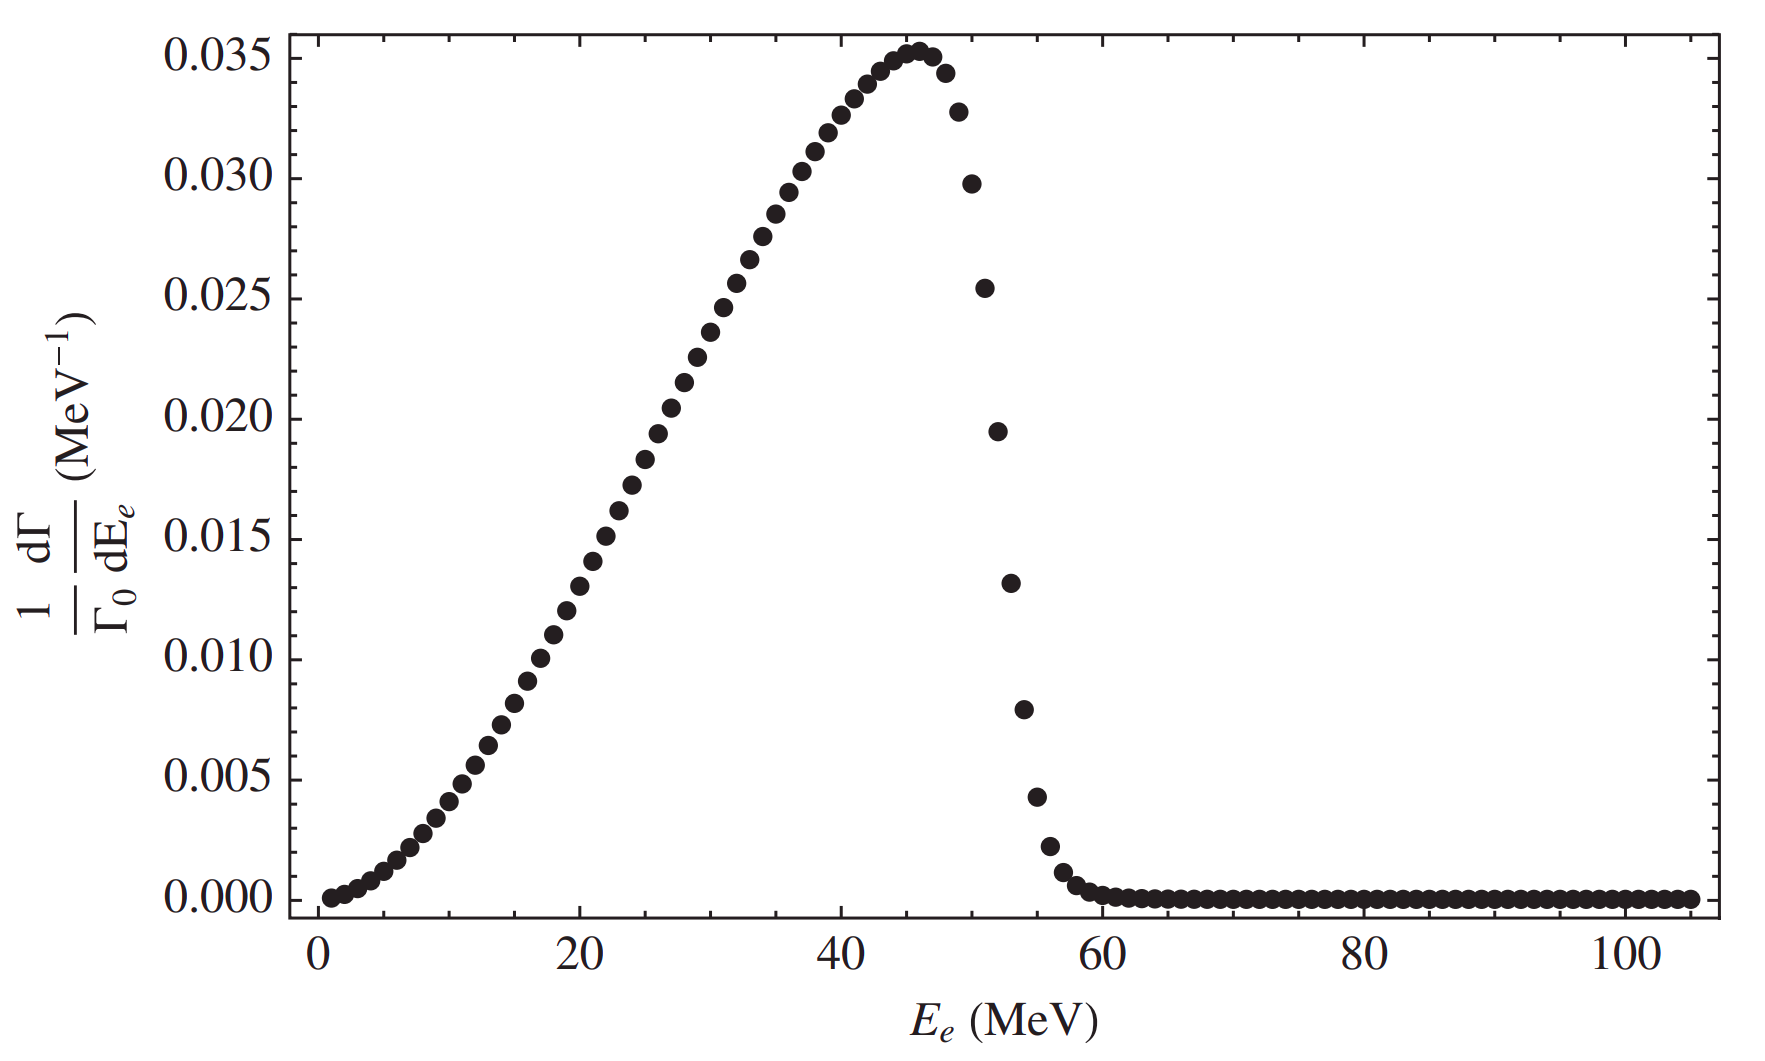
\includegraphics[scale = 0.18]{figures/png/Screenshot_20240222_175415.png}
         \subcaption{Linear scale.}
         \label{fig:linearscalemichel}
     \end{subfigure}
     \begin{subfigure}[b]{0.7\linewidth}
         \centering
         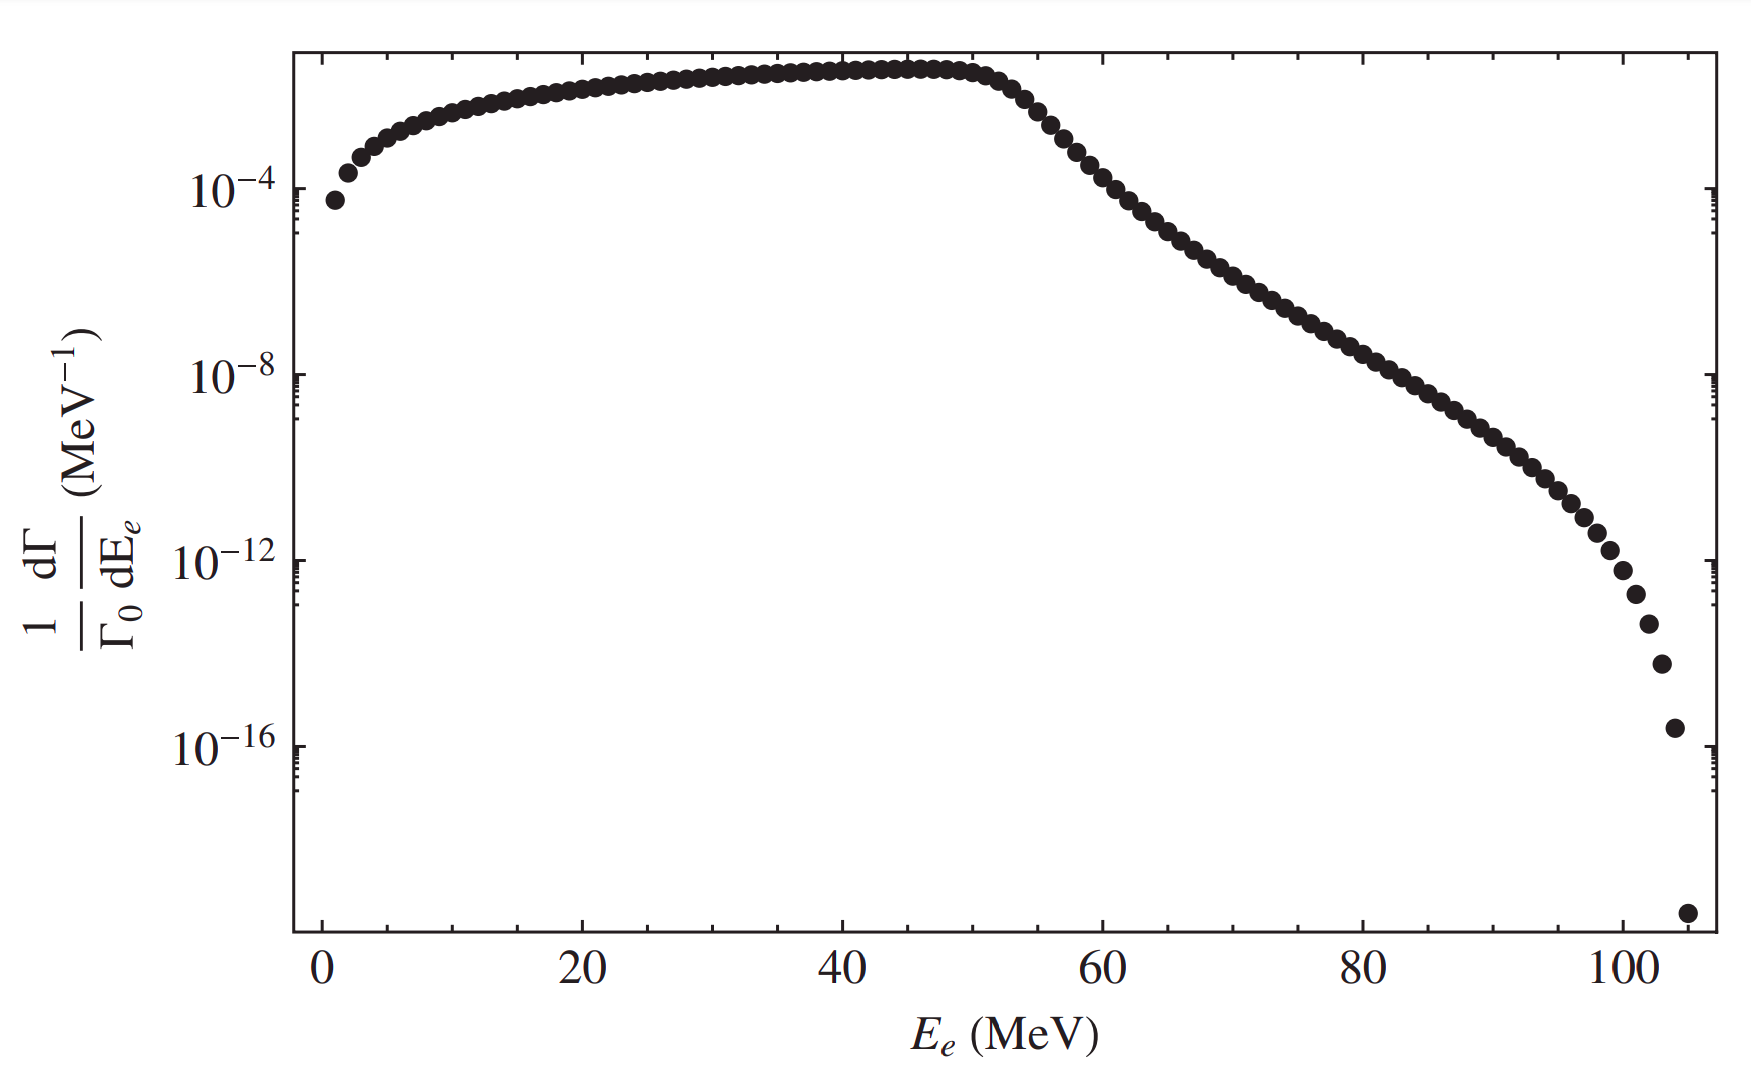
\includegraphics[scale = 0.18]{figures/png/Screenshot_20240222_175446.png}
         \subcaption{Logarithmic scale.}
         \label{fig:logscalemichel}
     \end{subfigure}
     \caption[Decay-in-orbit spectrum on aluminium.]{
       Decay-in-orbit electron spectrum on Al \cite{PhysRevD.84.013006}.}
        \label{fig:michel}
\end{figure}

\begin{figure}[!h]
\centering
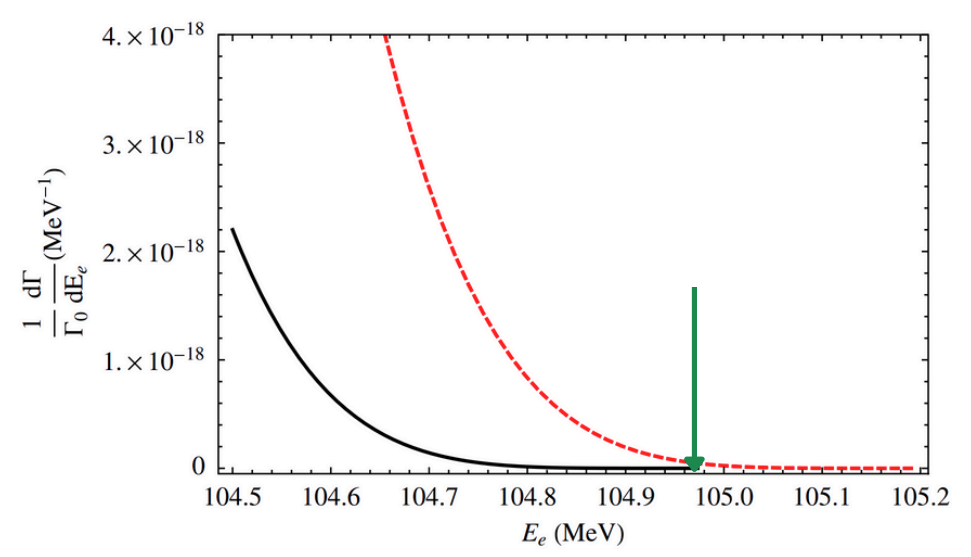
\includegraphics[width =0.55\textwidth]{figures/png/Screenshot_20240909_141143.png}
\caption[The electron energy spectrum near to the endpoint.]{The electron energy spectrum near to the endpoint. The black line 
represents the Michel spectrum w/o the nuclear recoil, while the red 
dashed line takes into consideration the recoil of the Al nucleus 
\cite{PhysRevD.84.013006}. The green arrow shows the spectrum end at 104.973 MeV.
}
\label{fig:micheldiff}
\end{figure}


\paragraph{Radiative Muon Capture}
The Radiative Muon Capture (RMC) is a muon capture with emission of an energetic photon.

In the process $\mu^- N \rightarrow\gamma \nu_\mu N'^* $, 
the photon can either be real or virtual. The photon, interacting with matter or 
undergoing pair production, can produce electrons with energies close to $E_{CE}$, 
introducing background to the experiment. The emitted photon's energy follows 
a spectrum, with its maximum energy, denoted as the kinematic limit $k_{max}$, 
determined by the equation \cite{bartoszek2015mu2e}:

\begin{equation}
k_{max} = m_\mu c^2 - |E_b| - E_{rec} - \Delta M ,
\end{equation}

where $E_b$ represents the muon binding energy on the initial nucleus, $E_{rec}$  
the recoil energy of the daughter nucleus and $\Delta M$ is the rest energy difference 
between the final and initial nuclei. This formula neglects higher order nuclear effects. 
RMC can be effectively mitigated in the Mu2e experiment by 
selecting Al as the ST material. The ST is selected so that the daughter nuclide of a muon-capture 
process of any kind is heavier than the original nuclide. For aluminum, the RMC photon 
endpoint energy is 101.9 MeV, approximately 3.1 MeV below the CE energy 
\cite{bartoszek2015mu2e}. 
The FWHM of the conversion peak is around 1 MeV, therefore the RMC background will be 
outside the signal region. However, the RMC background might distort the DIO spectra 
around 100 MeV range, making it difficult to extrapolate the high momentum end of the DIO spectrum. 
The RMC background will be determined from the positron data.


\subsubsection{Prompt processes}
This type of background sources can generate electrons at roughly the same time as 
the entering beam particles. There are four primary sources: radiative pion capture (RPC), 
pion decay-in-flight ($\pi$-DIF), muon decay-in-flight ($\mu$-DIF) and beam electrons.

\paragraph{Radiative Pion Capture}

Pions, reaching the ST and captured in Al can 
produce high-energy photons, i.e. $\pi^- N(A,Z) \rightarrow \gamma N ^* (A,Z-1)$. 
This process, called radiative pion capture,
has a branching ratio of $\sim 2\%$ \cite{PhysRevC.5.1867}.
Similar to RMC, the photon 
can internally convert into an electron-positron pair or be radiated as an on-shell photon 
and convert in the detector material producing an $e^+e^-$ pair. 
The resulting electrons contribute to the experiment background. 
Despite its similarity to RMC, RPC is a more challenging background to suppress due to 
the fact that the endpoint of the energy spectrum of photons, and consequently the 
resulting electrons, is not constrained by the rest energy of the muon.
The pion mass is 139.6 MeV, above the CE energy,
and the spectrum of the electrons resulting from RPC overlaps with the search region. 
The SINDRUM II results 
were limited by the pion-induced background and also by the low intensity of its muon 
beam \cite{SINDRUMII:2006dvw}. SINDRUM II used a primary proton beam with a 
frequency of one pulse every 19.75 ns, lasting approximately 0.3 ns. This interval 
between pulses was shorter than the 26 ns lifetime of pions \cite{zyla}, 
ensuring a consistent pion flux. To mitigate RPC, SINDRUM II made use of a degrader to suppress 
pions and a veto counter in the beam, resulting in less than one out of 10$^9$ pions reaching their 
target. However, given the more intense beam, the Mu2e experiment has to change the approach. 
Mu2e will suppress the RPC background by delaying the search window in time with respect
  to the incoming beam by several hundred nanoseconds \cite{universe9010054}. 
One important point to note is that the out-of-time protons could produce $late$ pions not rejected by the delayed timing window. 
Consequently, it is important for the pulsed beam to achieve a high extinction level. Further elaboration 
on the pulsed beam used in Mu2e will be provided in Section \ref{accel}.
\paragraph{$\pi$-DIF and $\mu$-DIF}
The pion decay-in-flight ($\pi$-DIF) and the muon decay-in-flight ($\mu$-DIF) 
exhibit quite similar characteristics. Free pions and muons can 
undergo electron decay while transitioning from the 
production target to the ST, through the processes 
$\mu^- \rightarrow e^- \nu_\mu \bar{\nu}_e$ and 
$\pi^- \rightarrow e^- \bar{\nu}_e$. In the center-of-mass 
frame of the initial particles, electrons originating 
from the first process exhibit an energy spectrum that 
reaches an endpoint of 52.8 MeV, while those from the 
second process have a consistent energy of approximately 
70 MeV. Since the pions and muons move at relativistic velocities, 
the energies (and momenta) of the resultant electrons are 
boosted. For instance, a muon with a momentum of around 
79 MeV/c or a pion with momentum close to 70 MeV/c can generate 
an electron with an energy of 105 MeV \cite{bartoszek2015mu2e}. 
Implementing a pulsed proton beam and using a delayed 
live window can help suppress background from $\pi$-DIF and 
$\mu$-DIF events. Particles with sufficient momentum 
to boost the daughter electrons to the concerning energies 
move quickly along the muon beamline and are gone by the 
time the live search window begins \cite{bobbb}. 


\paragraph{Beam electrons}\label{beamelectrons}
Other mechanisms generate electrons, both at the production target 
and along the muon beamline. For instance, neutral pions formed at 
the production target can decay in two photons, after which the 
photons can either create electron-pairs or interact with nearby 
materials to generate electrons. 
The beam electron background is suppressed by the delayed search timing window.


\subsubsection{Delayed processes from antiprotons}
Protons, at a given threshold, can generate antiprotons 
within the production target. This occurs through the 
process of antiproton production: $pp \rightarrow ppp\bar{p}$. 
If we consider that all four particles in the final state are 
at rest in the center of mass frame, the minimum kinetic energy 
needed for $p\bar{p}$ production can be found, which is 
approximately $6 m_pc^2 \sim 5.6$ GeV, where $m_p$ is the 
mass of the proton. In an ideal scenario, maintaining the 
beam energy below this threshold could enable us to avoid 
this background in the experiment. Unfortunately, the Mu2e 
proton beam goes beyond the threshold for antiproton production. 
The antiprotons are long-lived and massive. Antiprotons with 
momenta below 100 MeV/c travel at speeds less than 0.1$c$, 
requiring several $\mu$s to spiral from the production target 
to the ST \cite{bartoszek2015mu2e}. They have the correct 
charge and momentum to pass through the collimators placed 
between the production target and the ST. Annihilating or 
undergoing interactions with other materials, they have the 
capability to release a substantial amount of energy, generating 
numerous electrons. The delayed timing of 
such interactions is much longer than the muon lifetime, leading to a 
continuous flow of antiprotons reaching the ST. The pulsed beam and 
the delayed live window fail to suppress the antiproton background. 
The best approach is to prevent the antiprotons from reaching the 
region where the ST is located.
Two thin absorbers are positioned in 
the muon beamline to capture the antiprotons. Their design was 
developed to find a compromise between increasing antiproton 
absorption and decreasing muon beam loss. 

\subsection{Background estimates and signal sensitivity}
Mu2e run plan is divided in two different phases. Run I 
will take place in 2027, before a 2 years shutdown due to the 
planned accelerator upgrade for the long baseline neutrino 
program. In Run I phase one, a low intensity proton beam, 
$1.6 \times 10^7$ protons/pulse, will be used. In Run I 
phase two, the mean intensity will be increased up to $3.9 \times 10^7$ 
protons/pulse. As discussed in \cite{universe9010054}, during Run I, the 5$\sigma$ discovery sensitivity is 
$R_{\mu e}^{5 \sigma} = 1.2 \times 10^{-15}$, with a 
total expected background of 0.11$\pm$0.03 events. 
Reaching the 5$\sigma$ significance level requires 
observing 5 $\mu\rightarrow e$ events in the two-dimensional search window 
103.60 < $p$ < 104.90 MeV/c, 640 < $T_0$ < 1650 ns. In the 
absence of a signal, the expected upper limit is $R_{\mu e}$<$6.2 \times 10^{-16}$
at 90\% CL. 
The single event sensitivity (SES) is defined as
\begin{equation}
    SES \equiv \frac{1}{N_{POT} \cdot P_{\mu \ stop} \cdot \epsilon_{CE} \cdot BR_{capture}}
\end{equation} 
where $N_{POT}$ is the number of protons on target in the experiment, 
$P_{\mu \ stop}$ is the number of muons stopped on target per 
proton, $\epsilon_{CE}$ is the CE acceptance, which is a product 
of detector efficiency (dependent on the momentum signal region) 
and fraction of muons interacting in the live time window and 
$BR_{capture}$ is the branching ratio of muon captures, which 
is 60.9\%. The optimized Mu2e signal window corresponds to a 
SES of $2.3 \times 10^{-16}$. The background estimates after 
the sensitivity optimization are summarized in Table \ref{tab:summarybkg}.

Figure \ref{fig:sensitivity} shows the momentum and time distributions 
for CE signal and background processes corresponding to the optimized 
signal window for Run I. A detailed analysis and an estimate of the Mu2e 
expected backgrounds for Run I can be found in \cite{universe9010054}.
\begin{center}  
\begin{table}[!h]
\centering
\renewcommand{\arraystretch}{1.2}
\begin{tabular}{| c | c |}
\hline
\textbf{Channel} & \textbf{Mu2e Run I}\\
\hline
SES & 2.4 $\times \ 10^{-16}$ \\
\hline
Cosmic rays & 0.046 $\pm$ 0.010 (stat.) $\pm$ 0.009 (syst.) \\
DIO & 0.038 $\pm$ 0.002 (stat.) $ ^{+ \ 0.025} _{- \ 0.015}$ (syst.)\\
Antiprotons & 0.010 $\pm$ 0.003 (stat.) $\pm$ 0.010 (syst.) \\
RPC in-time & 0.010 $\pm$ 0.002 (stat.) $ ^{+ \ 0.001} _{- \ 0.003}$ (syst.)\\
RPC out-of-time & (1.2 $\pm$ 0.1  (stat.) $ ^{+ \ 0.1} _{- \ 0.3}$ (syst.)) $\times$ $10^{-3}$ \\
RMC & $<$ 2.4 $\times$ $10^{-3}$ \\
Decays in flight & $<$ 2 $\times$ $10^{-3}$ \\
Beam electrons & $<$ 1 $\times$ $10^{-3}$ \\
\hline
Total &  0.105 $\pm$ 0.032\\
\hline
\end{tabular}
\caption{Summary of the several background sources to 
the CE search as expected in Mu2e Run I \cite{universe9010054}. 
The Table also shows the corresponding SES. }

\label{tab:summarybkg}
\end{table}
\end{center}
\begin{figure}[!h]
\centering
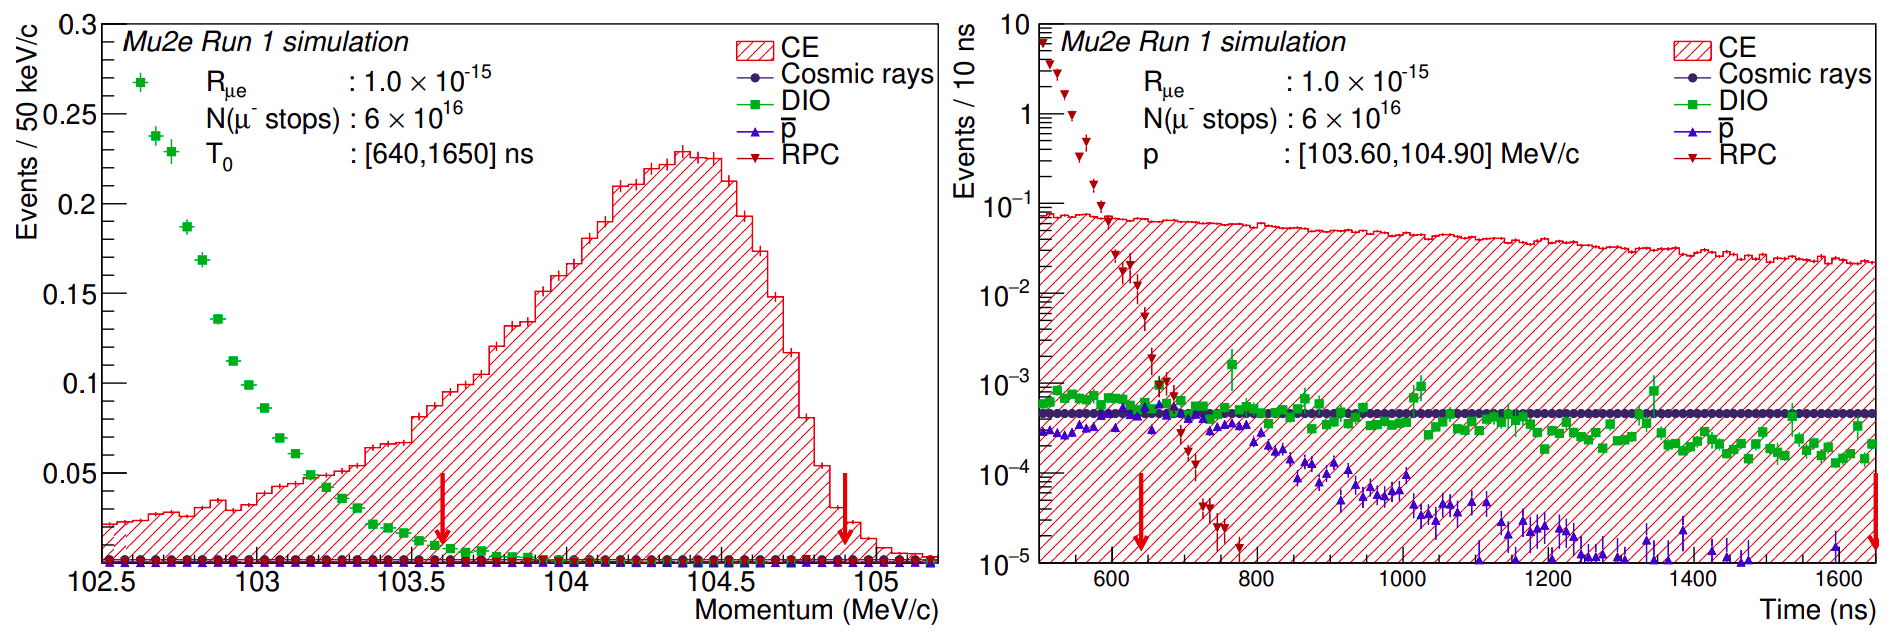
\includegraphics[width =0.93\textwidth]{figures/png/Screenshot_20240225_102708.png}
\caption[Mu2e simulated signal.]{Left: Momentum distribution of the CE signal and expected backgrounds. Right: Time distribution of the CE signal and expected backgrounds. The arrows show the signal region selected for the analysis, 103.60 $< \ p \ < $ 104.90 MeV/c and 640 $< \ T_0 \ < $ 1650 ns, Section \ref{pulsedprotonbeam}. The CE signal distributions correspond to $R_{\mu e} = 1 \times 10^{-15}$ \cite{universe9010054}.}
\label{fig:sensitivity}
\end{figure}
\section{Experimental setup}\label{setup}
Figure \ref{fig:mu2escheme} shows a schematic overview 
of the Mu2e experiment. The experiment uses 
a solenoid system to generate magnetic fields essential 
for its operations. The Production Solenoid (PS) surrounds 
the production target, while further downstream, the 
Transport Solenoid (TS) provides the magnetic field for 
the muon beamline. The TS, configured in an S-shape, 
incorporates collimators and proton absorbers. The ST is 
located at the beginning of the Detector Solenoid (DS). 
Proton absorbers surround the ST, not shown in the picture. 
The tracker and the calorimeter are housed in the DS, 
enabling momentum measurement and particle identification. 
Additionally, a Stopping Target Monitor (STM) positioned 
downstream at the DS's end, not shown, measures the rate of muons stopped in the ST.
Also not shown 
in the picture is the Mu2e CRV system which 
surrounds the DS and half of the TS. In the next sections, a 
more detailed description of systems of the Mu2e experiment will be given.
\begin{figure}[!h]
\centering
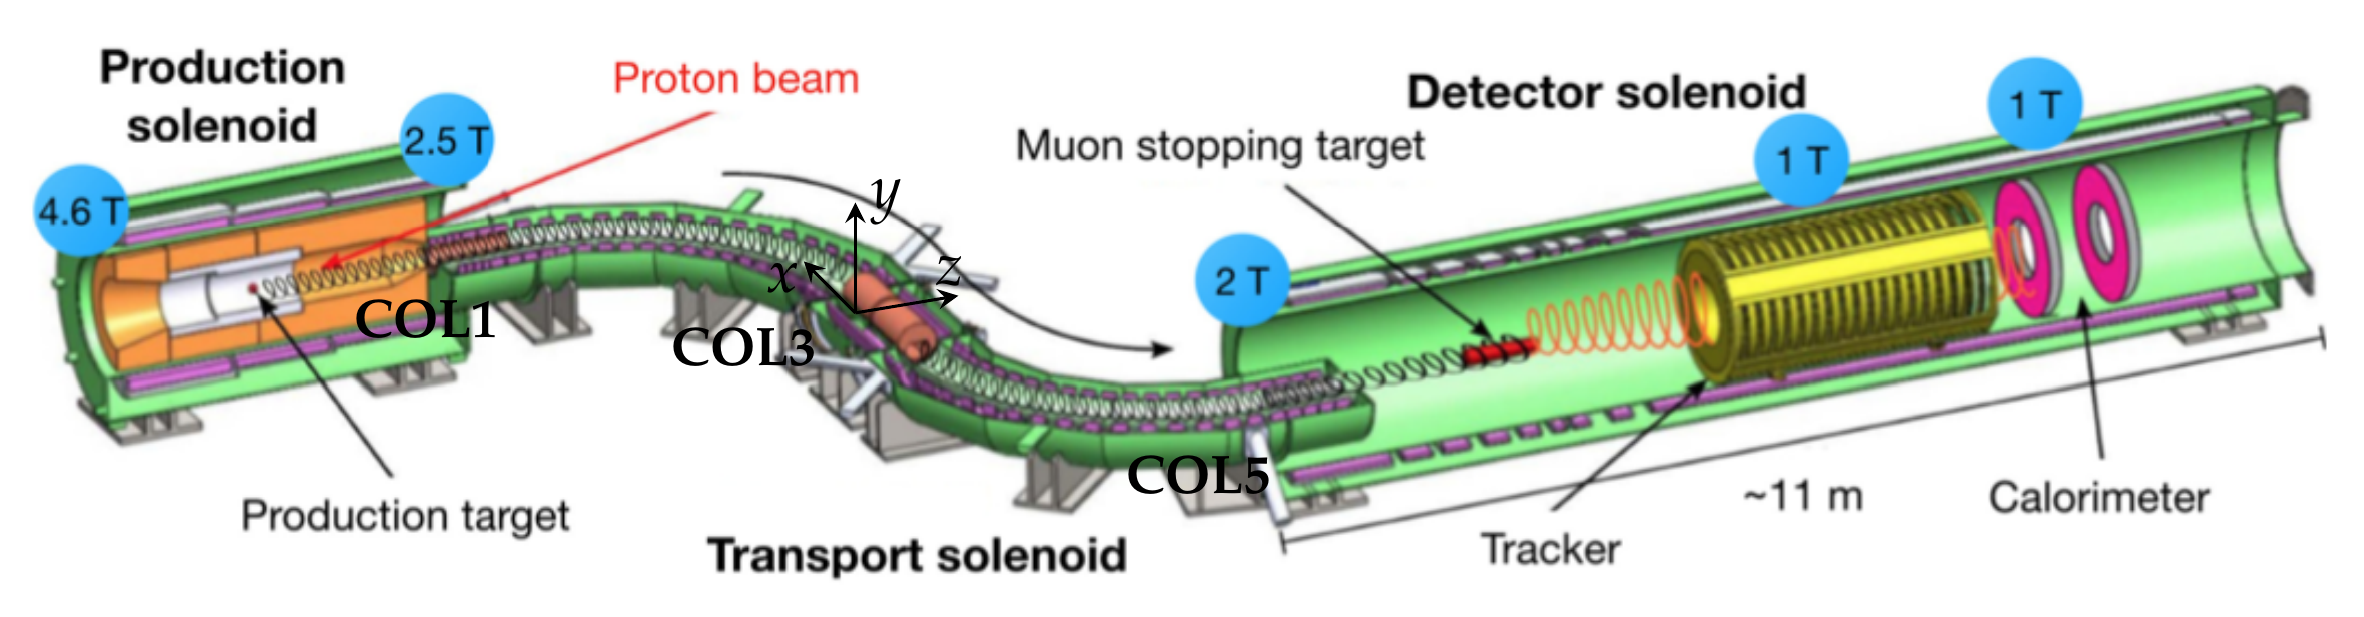
\includegraphics[width =\textwidth]{figures/png/Screenshot_20240301_143105.png}
\caption[The Mu2e apparatus.]{Schematic view of the Mu2e apparatus. The center 
of the Mu2e reference frame is located at the COL3 collimator center, its $y$-axis 
points upwards, the z-axis is parallel to the DS axis and points downstream, and 
the $x$-axis completes the right-handed reference frame \cite{universe9010054}.}
\label{fig:mu2escheme}
\end{figure}
\section{Accelerator system and the proton beam}\label{accel}
\subsection{Pulsed proton beam}\label{pulsedprotonbeam}
As previously discussed in Section  \ref{backgrounds}, the Mu2e experiment uses a 
pulsed proton beam.

The 8 GeV, 8 kW beam originates from the Fermilab Booster \cite{PhysRevAccelBeams.20.111003}. 
The proton pulses are separated by 1695 ns. Figure \ref{fig:accell} 
illustrates the Fermilab accelerator facilities involved in generating and delivering 
the pulsed proton beam. The Fermilab Booster delivers 8 GeV protons in 20 batches 
throughout a 1.4 s Main Injector cycle at 15 Hz, as shown in Figure \ref{fig:deliver}. 
Thus, the accelerator timeline is described using a fundamental time unit of 1 tick that corresponds to 66.7 ms.

\begin{figure}[!h]
     \begin{subfigure}[b]{0.4\linewidth}
         \centering
         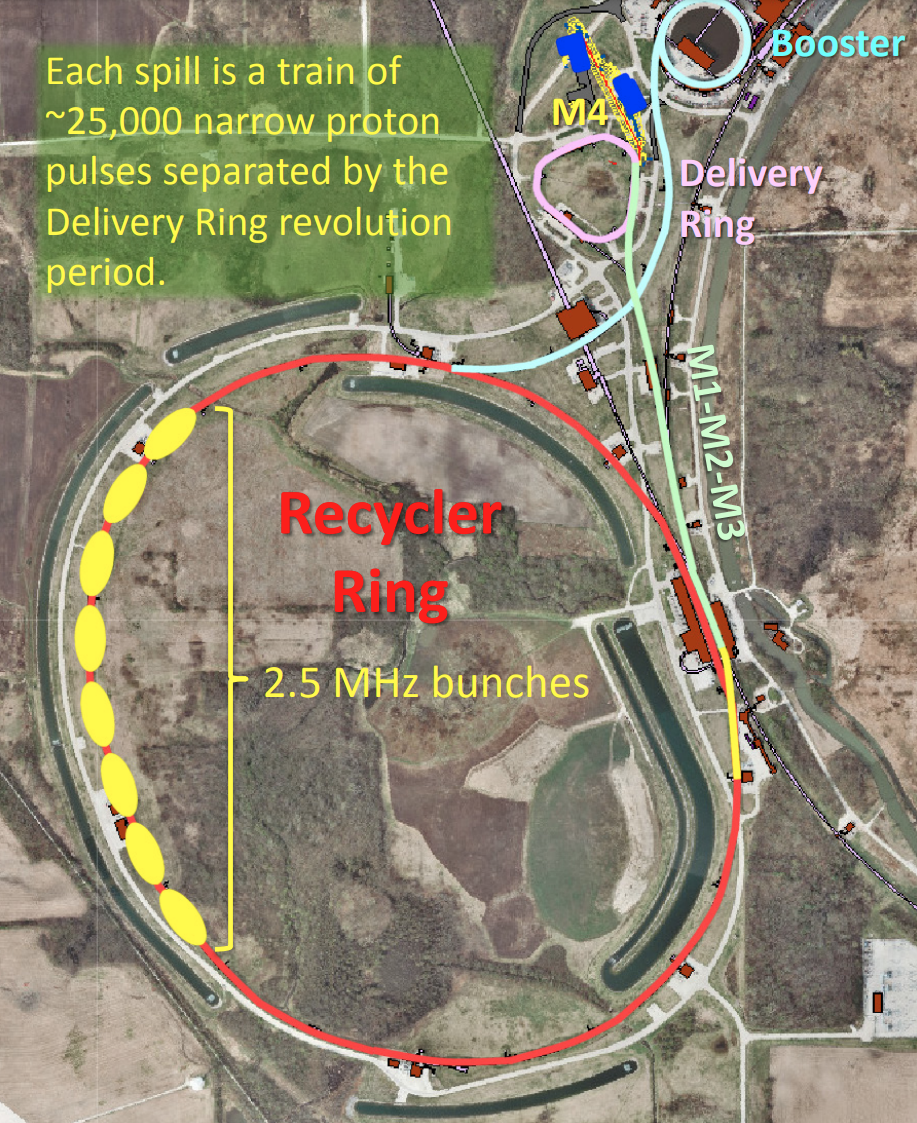
\includegraphics[scale = 0.3]{figures/png/Screenshot_20240301_151449.png}
         \subcaption{\centering Fermilab accelerator facilities involved in producing and delivering the pulsed proton beam.}
         \label{fig:accell}
     \end{subfigure}
     \begin{subfigure}[b]{0.7\linewidth}
         \centering
         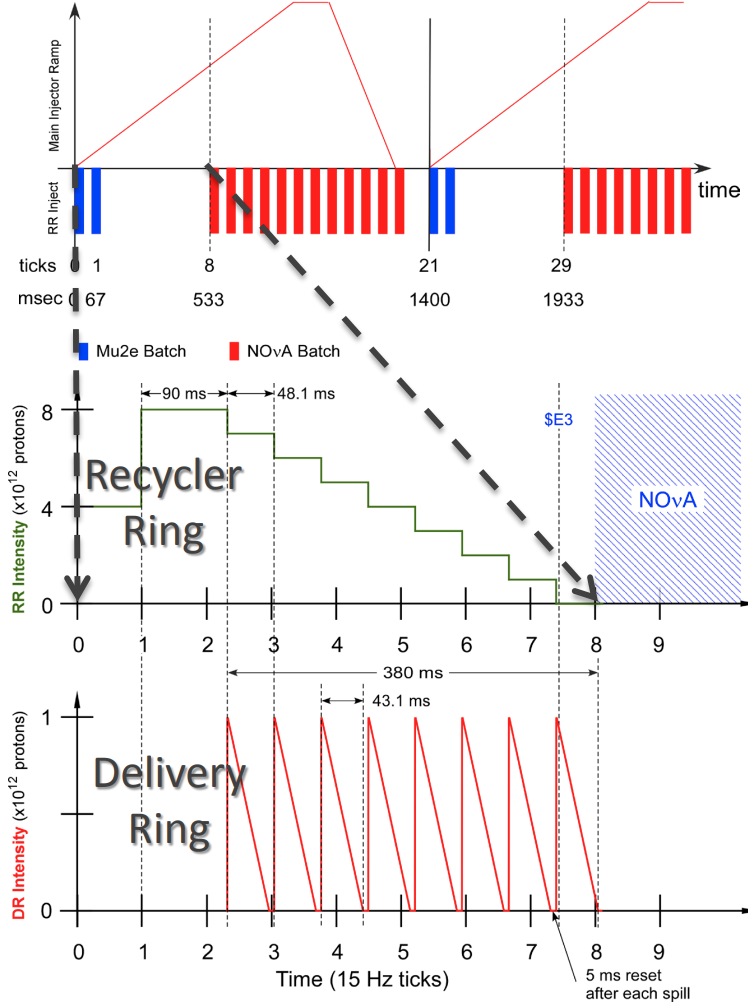
\includegraphics[scale = 0.39]{figures/png/Screenshot_20240301_151418.png}
         \subcaption{\centering Proton beam delivery to Mu2e.}
         \label{fig:deliver}
     \end{subfigure}
     \caption[The pulsed proton beam delivery.]{Pulsed proton beam delivery \cite{accelerator}.}
        \label{fig:three graphs1}
\end{figure}
The two Mu2e batches, represented by the two blue bars at ticks 1 (1BB) and 2 (2BB), are injected 
into the Recycler Ring, each containing $4 \times 10^{12}$ protons. The 
protons from these batches are reorganized within the Recycler using a 2.5 
MHz radio frequency (RF) system into 8 bunches. These bunches are then extracted 
individually from the Recycler and transported to the Delivery Ring every 48.1 ms, 
as shown in the middle part of Figure \ref{fig:deliver}. Once inside the Delivery 
Ring, a single bunch of $1 \times 10^{12}$ protons undergoes gradual extraction. 
This process results in the extraction of a small fraction of the bunch per revolution, 
delivered to the Mu2e experiment. The complete bunch is extracted over a span of 43.1 ms, 
across $\sim$25000 turns around the Delivery Ring, as shown in the bottom part of Figure \ref{fig:deliver}.
\begin{figure}[!h]
\centering
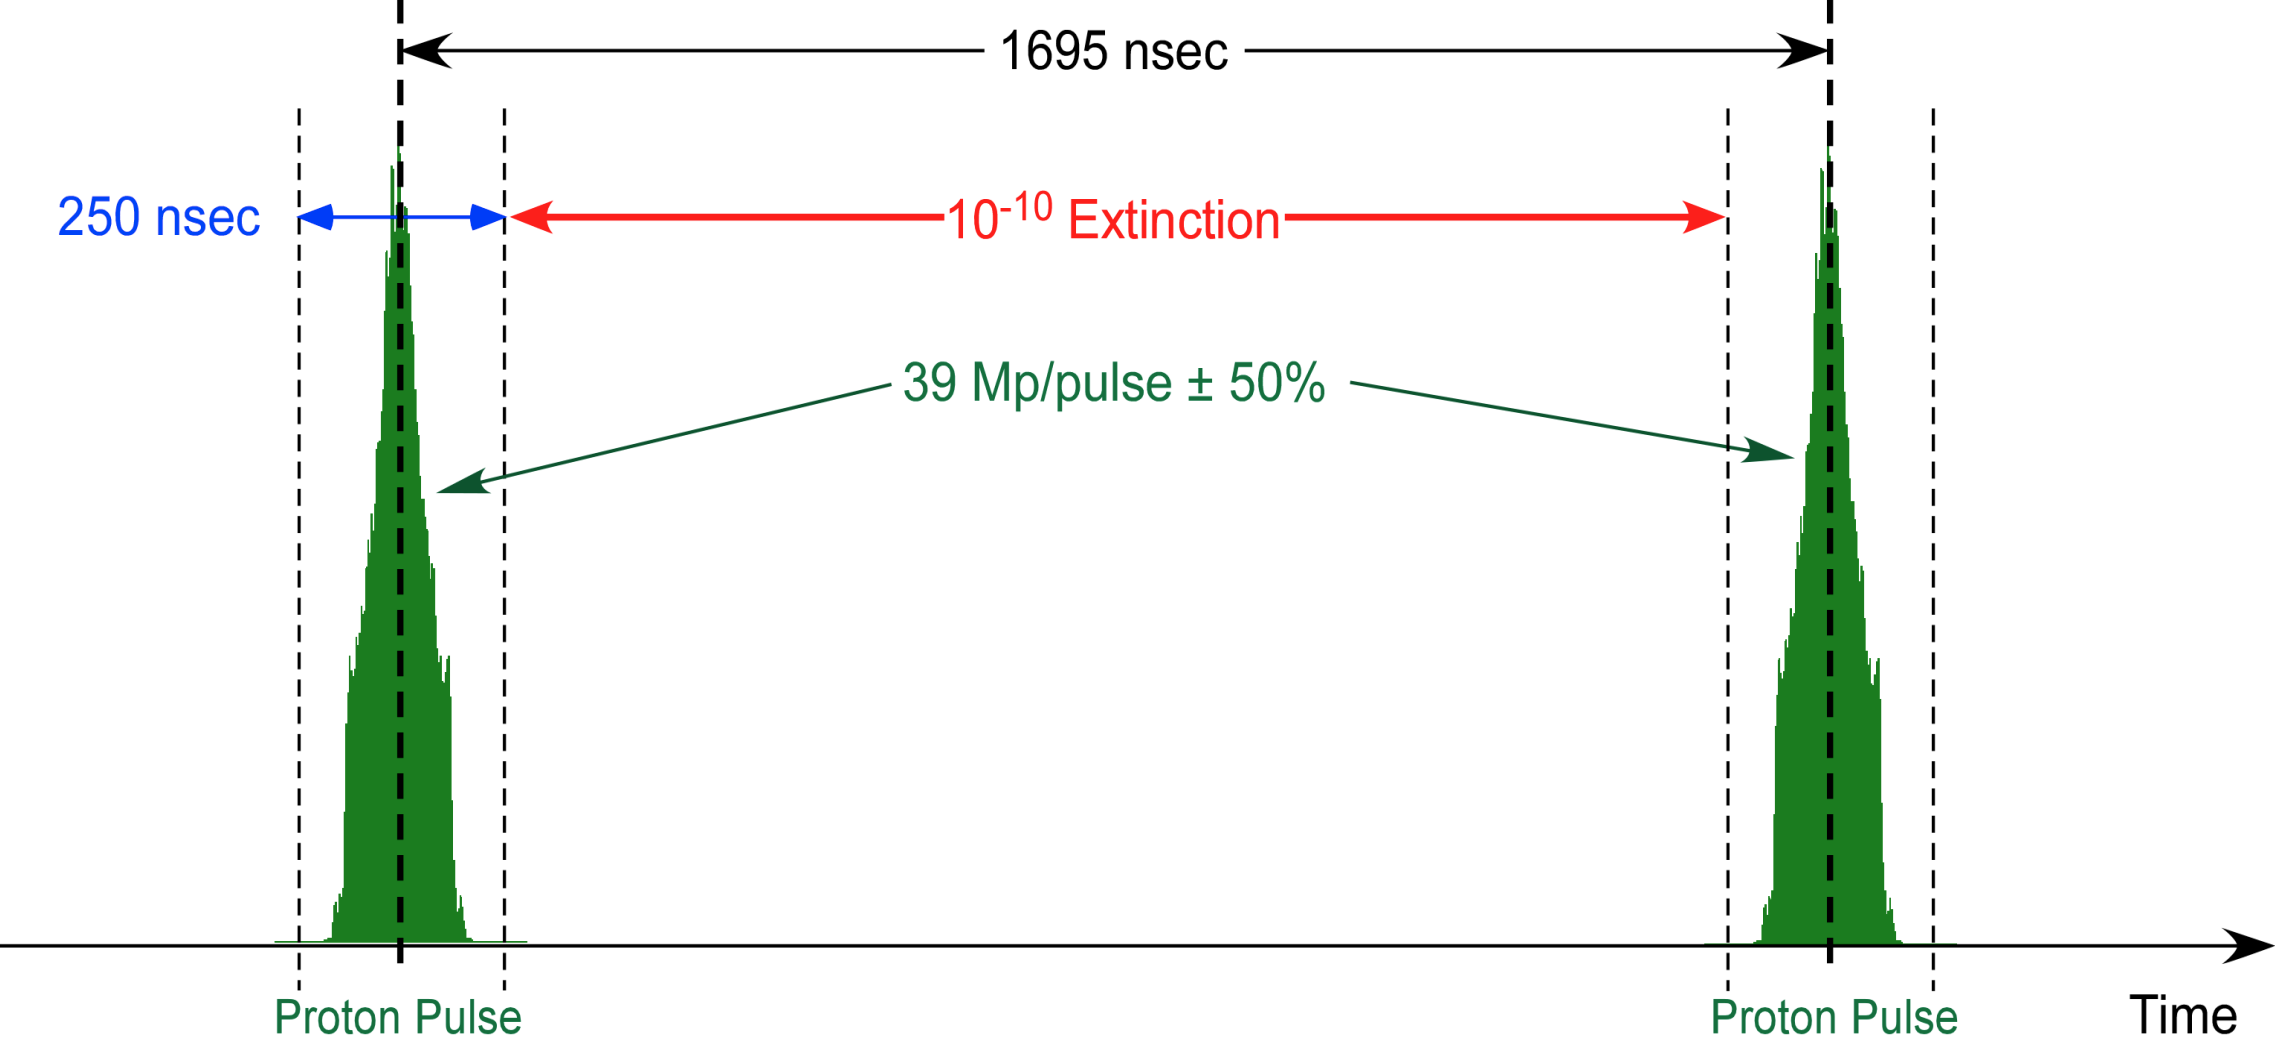
\includegraphics[width =0.8\textwidth]{figures/png/Screenshot_20240301_151148.png}
\caption[Proton beam profile.]{Proton beam profile at the Mu2e Proton Target \cite{accelerator}.}
\label{fig:beamprofile}
\end{figure}
Figure \ref{fig:beamprofile} illustrates the temporal 
profile of the beam at the PT. Consecutive 
proton pulses are spaced by 1695 ns. Each pulse lasts for 
250 ns and contains $(3.9 \pm 2.0 )\times 10^7$ protons. 
The 1695 ns pulse separation is highly advantageous for 
the Mu2e experiment. Figure \ref{fig:beamwindow} shows the beam pulse, 
the simulated pion flux, the muon capture rate on the ST 
and the muon decay rate. The active window for detecting 
CEs begins at $\sim$640 ns and extends for more or less 1 
$\mu$s. 

\begin{figure}[!h]
\centering
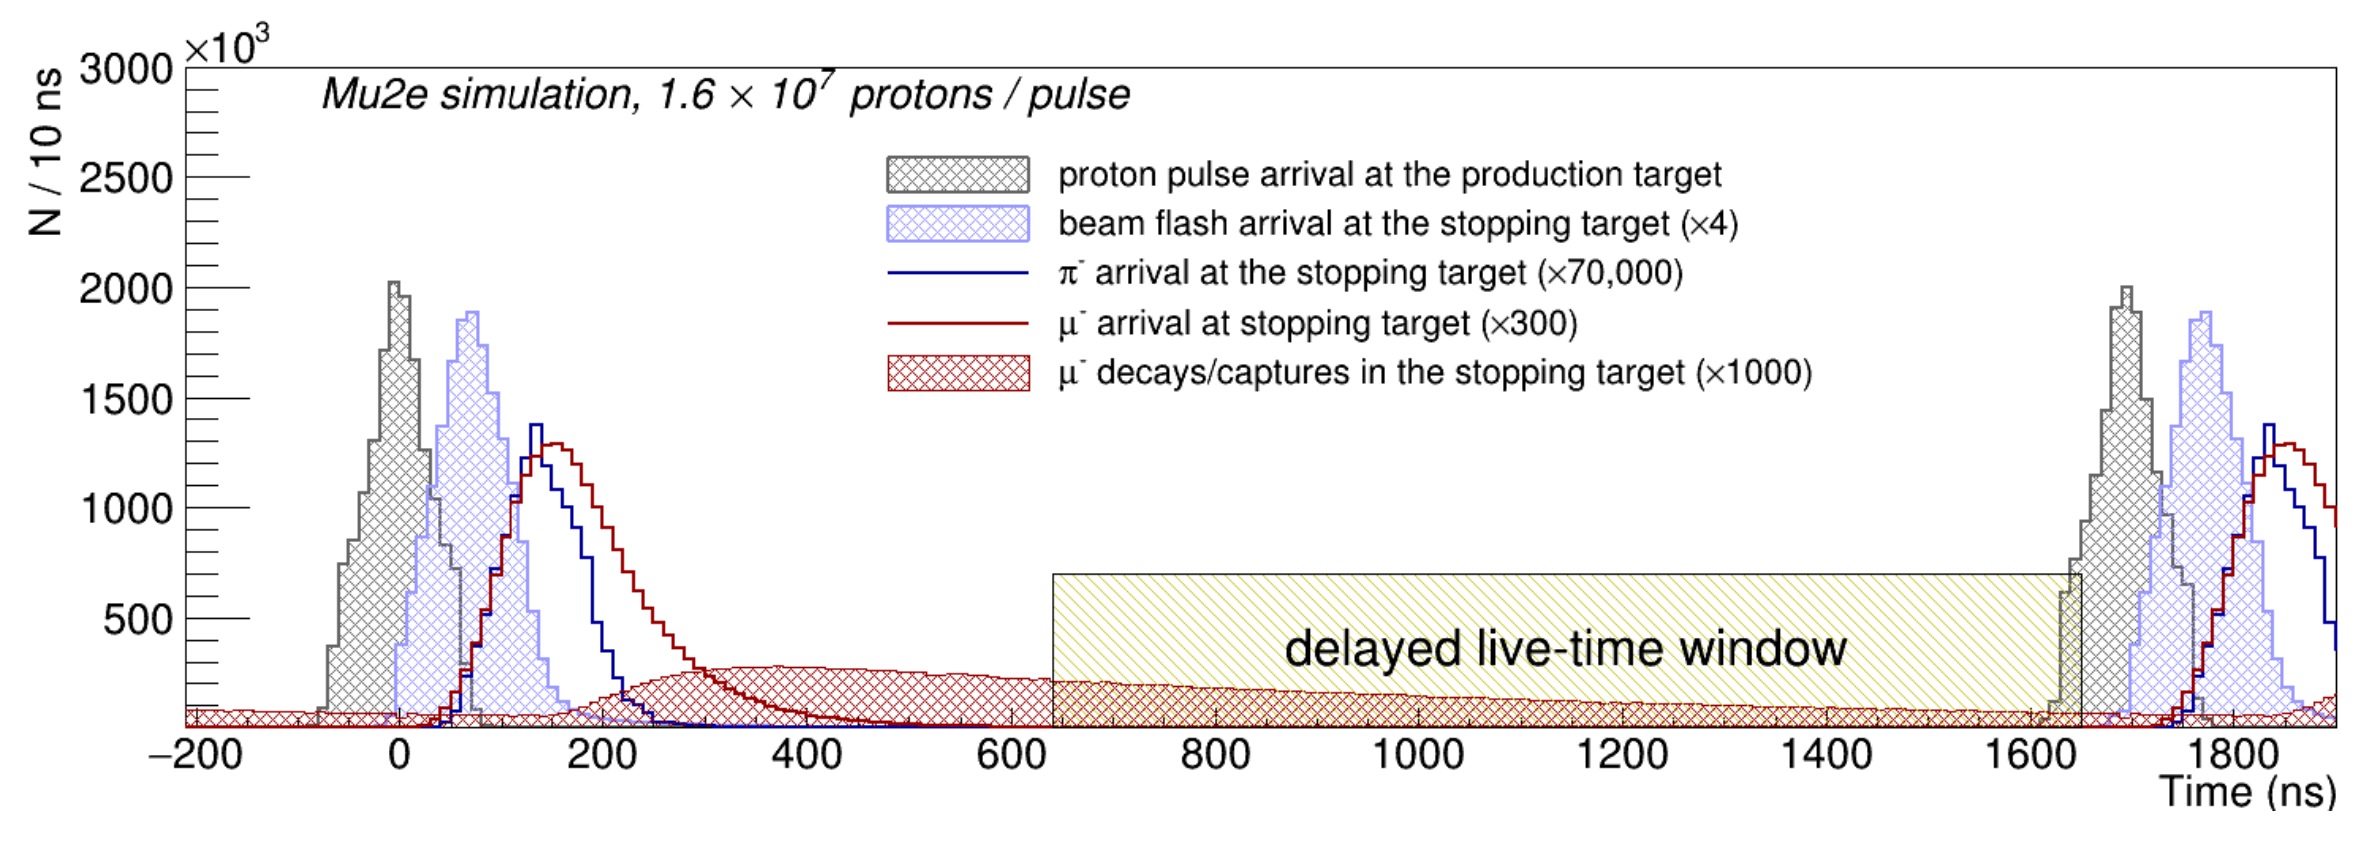
\includegraphics[width =0.9\textwidth]{figures/png/Screenshot_20240301_164649.png}
\caption[The Mu2e beam timing]{The Mu2e beam timing: the proton pulses arrive at the production solenoid every 1695 ns. A delayed live-time window can suppress the beam-related background \cite{universe9010054}.}
\label{fig:beamwindow}
\end{figure}
\subsection{Proton beam extinction and Extinction Monitor}
As mentioned in the previous section, the Mu2e experiment 
requires the extinction level of the incoming proton beam, to reduce backgrounds caused by out-of-time protons. 
The extinction rate, defined as the ratio between the 
number of out-of-time protons and the number of the in-time protons, should be lower than $10^{-10}$ \cite{bartoszek2015mu2e}. The structure of the beam 
leads to an extinction level $2.1 \times 10^{-5}$. To take into account the fact that some beam will 
leak out of two consecutive proton pulses, an Extinction 
Insert is deployed in the M4 beamline between the Delivery Ring and the Mu2e experiment.
The out-of-time beam particles are swept into a collimator system by an oscillating dipole, called AC dipole. These AC dipole 
offers an additional 
extinction factor of $5\times 10^{-8}$, reducing the 
overall extinction to $1.1 \times 10^{-12}$, leaving a margin of 10$^2$ \cite{accelerator}. An 
Extinction Monitor is positioned downstream of the 
production target along the proton beamline, as shown in Figure \ref{fig:extintion}. It monitors the 
extinction level of the proton beam and delivers a measurement with an accuracy of 10\%.

The Extinction Monitor consists of a collimator and magnetic filter 
system, a pixel telescope, a system of trigger scintillators and a range-stack. The collimator and 
magnetic filter system transport a small quantity of 
the particles generated at the production target to the Extinction Monitor. The pixel telescope 
tracks the trajectory of charged particles coming from 
the collimator. The pixel telescope consists of a permanent magnet and 8 scintillators, as shown 
in Figure \ref{fig:extintionmonitor}. The system uses a 
permanent magnet to separate two sets of four scintillator planes, allowing for momentum measurements 
of entering particles. The range stack is located further 
downstream from the pixel telescope. Steel absorber plates separate scintillators, distinguishing 
between hadrons and muons based on their penetrating capacity.
\begin{figure}[!h]
\centering
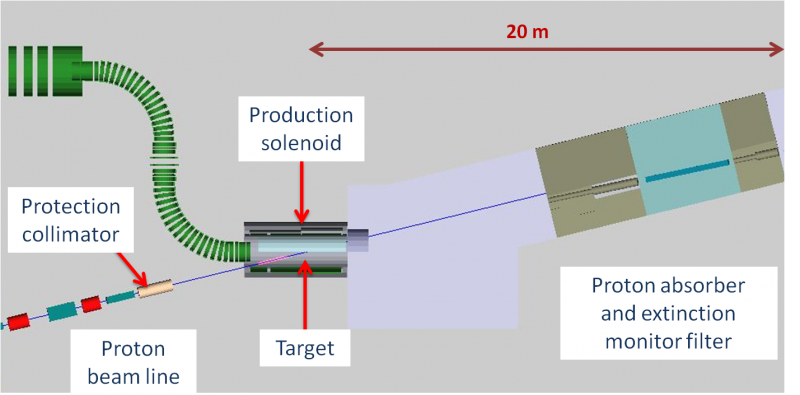
\includegraphics[width =0.8\textwidth]{figures/png/800px-Extinction_filter.png}
\caption[The Extintion Monitor location.]{The Extinction Monitor is located downstream of the
production target \cite{Prebys:IPAC2015-THPF121}.}
\label{fig:extintion}
\end{figure}
\begin{figure}[!h]
\centering
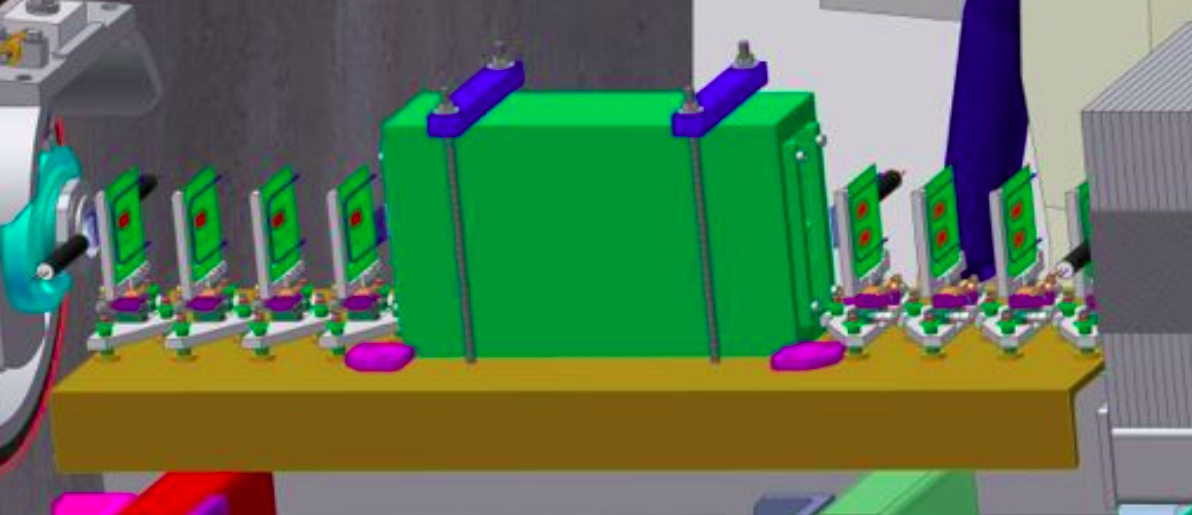
\includegraphics[width =0.7\textwidth]{figures/png/Screenshot_20240306_184720.png}
\caption[The Extintion Monitor.]{The tracking spectrometer of the Mu2e experiment, consisting of eight planes of pixel detectors and a permanent magnet spectrometer \cite{Prebys:IPAC2015-THPF121}.}
\label{fig:extintionmonitor}
\end{figure}
\subsection{Production Target}
The Mu2e production target (PT) is made of tungsten. 
The material was chosen because of its high 
melting point (3422 °C) and excellent resistance to deformation and corrosion.

It is positioned in the middle of the PS bore \cite{bartoszek2015mu2e}.
The tungsten core is embedded in a \textit{bicycle wheel} frame, 
suspended by the spokes.
The current design of the PT, shown in Figure \ref{fig:PT}, 
has circular rings at the end and its segmented core provides a better temperature 
dissipation. This design is expected to last for more than one year. The PT provides a muon yield of 0.0016 $\mu$/proton \cite{PT}.
\begin{figure}[!h]
    \centering
    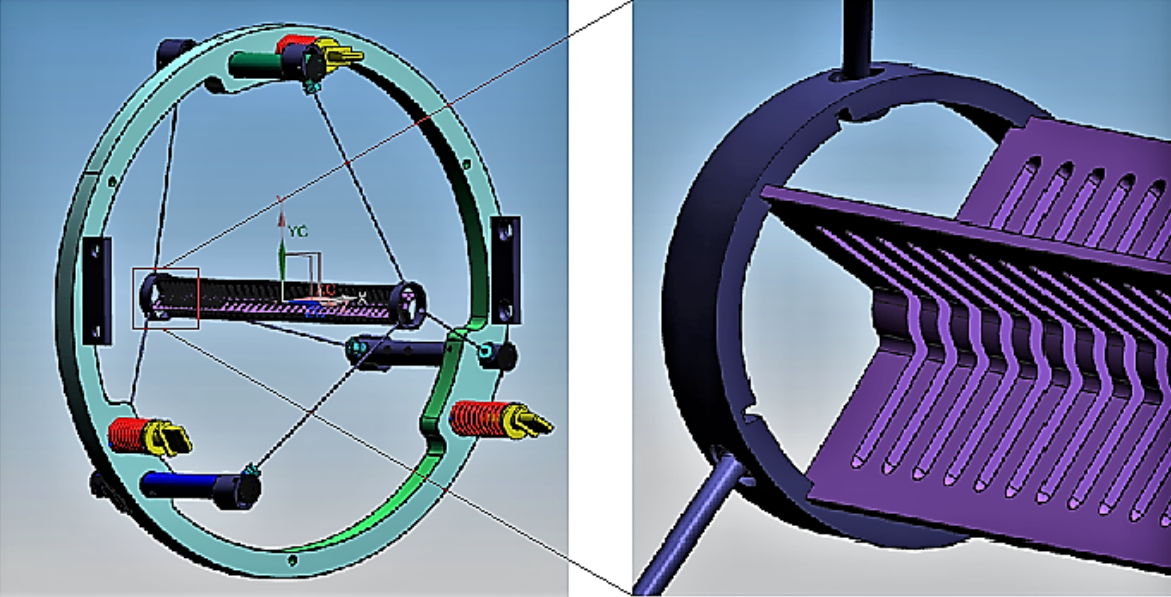
\includegraphics[width =0.7\textwidth]{figures/png/Screenshot_20240706_114229.png}
    \caption[The Production Target design.]{The design of the PT. Left: bicycle wheel 
      structure with the PT at the
    center. Right: zoom on the tungsten target.}
    \label{fig:PT}
\end{figure}

\section{Solenoids}
The principle of the Mu2e experiment is to use a sophisticated magnetic system
to form the high-intensity muon beam by collecting and filtering the particles emerging from the PT. 
It is composed of three parts: the \textbf{Production Solenoid} (PS), 
the \textbf{Transport Solenoid} (TS) 
and the \textbf{Detector Solenoid} (DS), shown in Figure \ref{fig:mu2escheme}. 
Each one is made of superconducting 
coils wound with aluminum stabilized Nb-Ti Rutherford cables.

The resulting magnetic field varies from 4.6 T at the upstream end of the PS 
to 1 T at the downstream end of the DS. 
The muons are guided towards the ST and the DS by lowering the magnetic field. 
Local magnetic field minima are avoided to avoid trapping particles in these areas. 
In the PS, the magnetic field decreases from 4.6 T to 2.5 T at the entrance of 
the TS. The large gradient helps to collect the secondary pions and muons and to 
direct them towards the DS. The magnetic field across the S-shaped TS changes its 
value only by a factor of 0.5 T. The shape of the TS allows to select charged particles 
and its dimension was set to avoid transmitting 
particles with large momentum. These particles either spiral with a large helical 
radius (large initial momenta perpendicular to the field) or cannot create an 
S-shaped bend (large initial momenta parallel to the magnetic field), resulting 
in collisions with solenoid walls or collimators. As particle drifts in the solenoid field is dependent on the particle charge,  
positively and negatively charged muons 
drift in opposite vertical directions and are separated, as explained in Appendix 
\ref{appendix1}. In the upstream part of the TS, Figure 
\ref{fig:collimators}, the positive (blue) and negative (red) muons 
are deflected downwards and upwards respectively. Positive muons are stopped in 
collimators COL3u and COL3d. The TS is long enough for pion decay, suppressing 
RPC backgrounds.
The magnetic field in the first half of 
the DS is reduced from 2 T to 1 T. In a smoothly gradient field, the adiabatic 
invariance of the magnetic flux can be used. Assuming a constant $p^2_\perp/B$, there is:
\begin{equation}
    v^2_{\parallel}=v^2_0-v^2_{\perp 0}\frac{B(z)}{B_0}
\end{equation}
Here, $\perp$ is referred with respect to the magnetic field $B$ and $\parallel$ is 
referred to the $z$ direction. The subscript 0's indicates the initial state. 
The gradient pitches electrons forward into the tracker's acceptance. 

The second half of the DS containing the tracker and the calorimeter has a 
uniform magnetic field of 1 T.

\begin{figure}[!h]
\centering
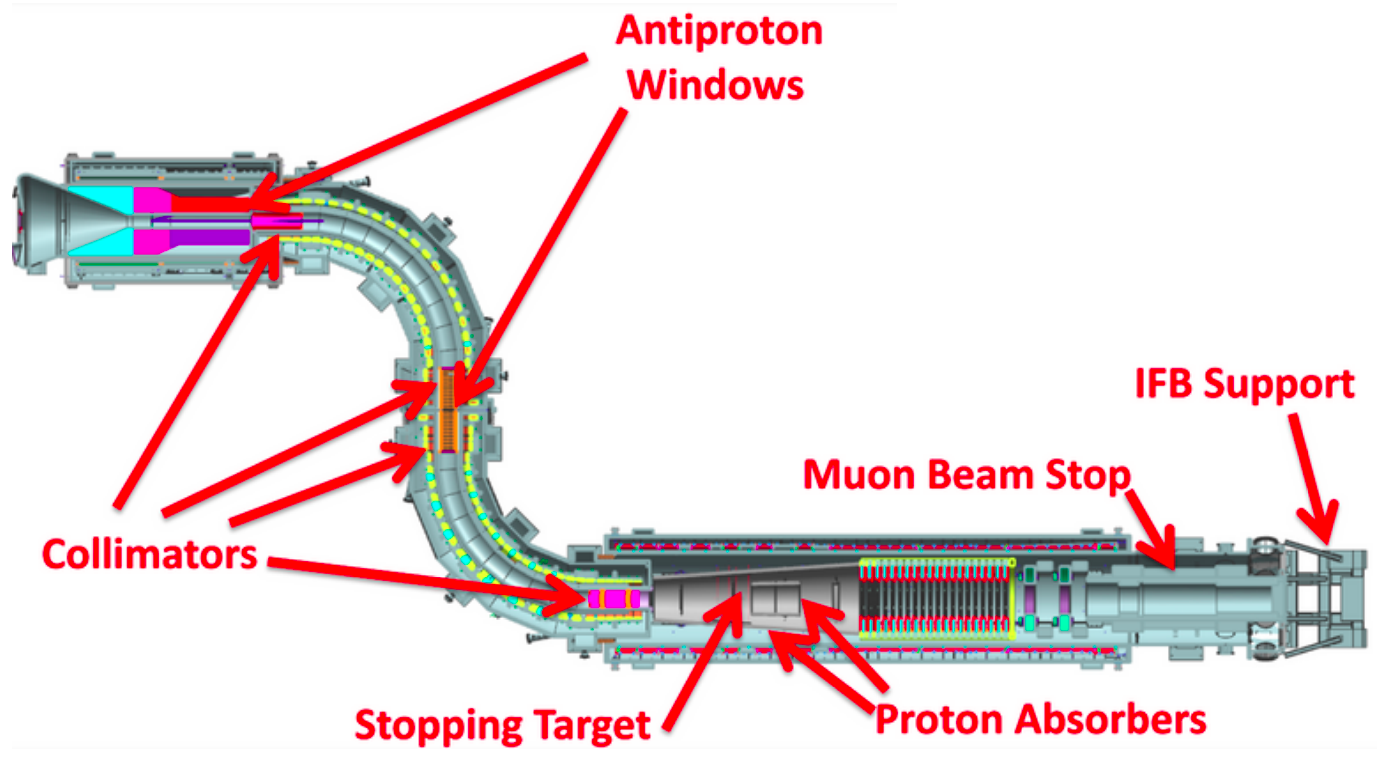
\includegraphics[width =0.7\textwidth]{figures/png/Screenshot_20240303_152845.png}
\caption[The muon beamline.]{The muon beamline, composed of the Production Solenoid (PS), 
the Transport Solenoid (TS) and the Dector Solenoids (DS) \cite{ginther}. 
}
\label{fig:muonbeamline}
\end{figure}


\subsection{The Production Solenoid}
The Production Solenoid (PS) (4 m long), shown in Figure 
\ref{fig:PS}, collects pions, 
kaons generated by the interactions between the 8 GeV 
proton beam and the production target. 
It is composed of Nb-Ti superconducting cables stabilised with Al 
and cooled by liquid helium. To avoid damages to the 
superconducting cables and
to the cooling system a bronze heat and radiation shield 
is built inside the solenoid. 
The position and shape of both the target and the magnetic 
field have been optimized to
maximize the production and collection of the 
desired particles: backwards pions and
muons. This choice was made to avoid the overwhelming
flux of particles (neutrons, photons, electrons and 
positrons from photon conversions) produced in the forward 
direction and the leftover incoming protons. 
The magnetic field is 4.6 T at the end of the PS and 
decreases almost linearly to 2.5 T at the
junction with the TS.
The magnetic field gradient allows to collect also part of the particles 
emitted along the proton beam direction, improving 
the stopped muon and pion yield.


\begin{figure}[!h]
    \centering
    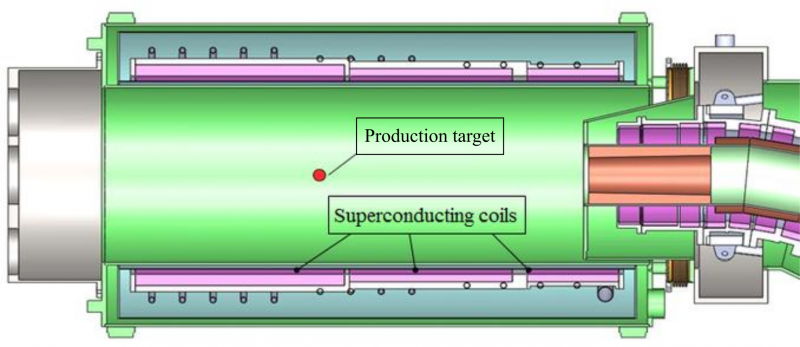
\includegraphics[width =0.7\textwidth]{figures/png/800px-Production_solenoid.png}
    \caption[The cross-section of the production solenoid.]{Cross-section of the production solenoid \cite{6376120}.
    The production target is placed approximately at the center of the superconducting coils.}
    \label{fig:PS}
    \end{figure}
\subsection{The Transport Solenoid}
The S-shaped TS is composed of a series of wide aperture superconducting
solenoid rings. It also contains a set of collimators and absorbers 
to provide charge and 
momentum selection and reduce the flux of antiprotons.
A thin window assembly is installed at the 
beginning of the TS and also between the rotatable collimators 
to absorb antiprotons in 
the beam. 

It is divided in five parts. 

The first one is called TS1 that contains the first collimator (COL1), 
Figure \ref{fig:collimatorsshape}, made of copper wedges. 
It filters particles from their momentum and reduces the 
radiation damage for coils of the 
upstream part of the TS (TSu). 

The TS2 contains a toroidal field in order to create a 
vertical displacement of the charged particles,
according to their charge and momentum.
Neutral particles, that are not sensitive to the magnetic 
field are not transported to the next section.

In TS3, negative muons are selected with two rotatable collimators (COL3u and COL3d, 
shown in Figure \ref{fig:collimatorsshape}). 
The rotatable feature allows selection of $\mu^-$'s instead of $\mu^+$'s, which can 
be used for detector calibration. 

The TS4 is the second toroid section of the TS and its role is 
to collimate the beams on the TS axis.

TS5 connects TS with DS and it contains a collimator (COL5), 
Figure \ref{fig:collimatorsshape}, made of polyethylene, 
which will serve as a shield from antiprotons.

It is linked to the DS 
and matches its field to provide the best beam transmission.


\begin{figure}[!h]
    \centering
    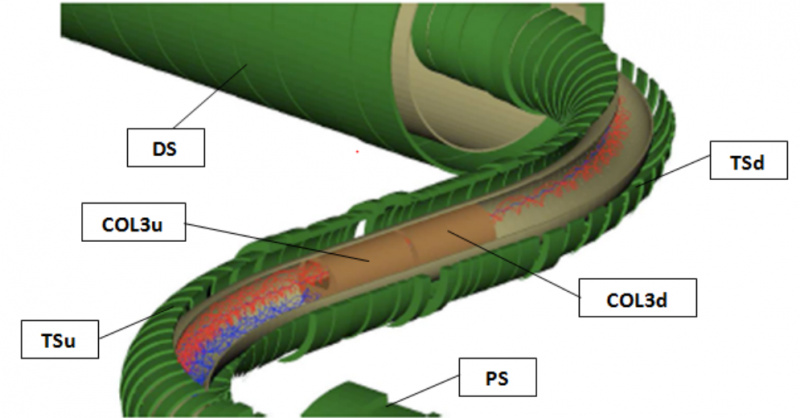
\includegraphics[width =0.7\textwidth]{figures/png/800px-MuonBeamlineCollimators2.png}
    \caption[The Transport Solenoid and the collimators.]{The schematic representation of the TS and the collimators COL3u and 
    COL3d showing the offset apertures in those collimators. The 
    upper spiraling negative muons (red) pass through the aperture while 
    the positive muons (blue) are stopped by these collimators \cite{tsview}.}
    \label{fig:collimators}
    \end{figure}
    \begin{figure}[!h]
        \centering
        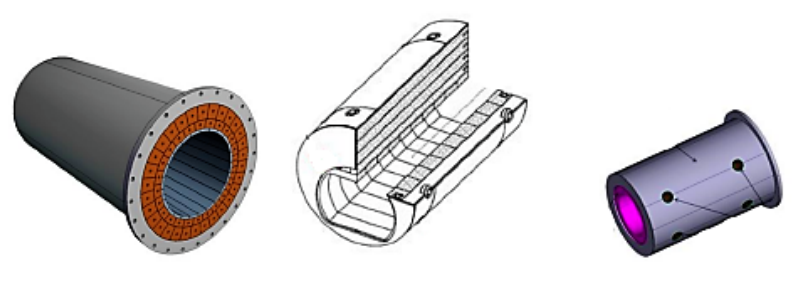
\includegraphics[width =0.7\textwidth]{figures/png/Screenshot_20240706_120535.png}
        \caption[The design of the collimators in the TS.]{Design of the collimators in the TS. From left to right: COL1, COL3u and COL3d
        and COL5.}
        \label{fig:collimatorsshape}
        \end{figure}

\subsection{The Detector Solenoid}\label{detectorsolenoid}
The DS, shown in Figure \ref{fig:DS}, is a cylindrical 
system of approximately 11 m in 
length and 2 m in radius, which houses the ST, 
the proton absorber, the tracker and the calorimeter. 
\begin{figure}[!h]
    \centering
    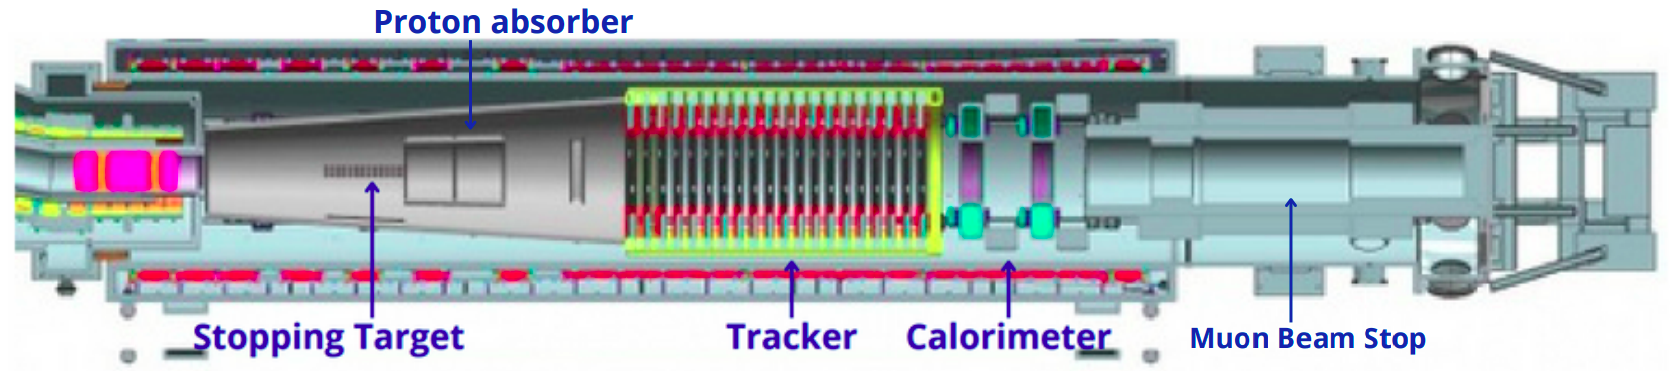
\includegraphics[width =0.8\textwidth]{figures/png/Screenshot_20240306_225639.png}
    \caption[The structure of the Detector Solenoid coils and cryostat.]{Overall structure of the DS coils and cryostat \cite{bobbb}.}
    \label{fig:DS}
    \end{figure}
The system is divided into two sections: a 4 
m gradient section following the TS, 
where the magnetic field decreases linearly from 2 T to 1 T, and a 6 
m spectrometer section. 

The gradient region drives the CE 
inside the tracker acceptance, while the low momentum particles 
are driven to the low radius region that is not covered by detectors.  

In the spectrometer region, the uniform magnetic field allows a precise 
measurement of the particle momentum. 

The DS is straight, differently from the COMET experiment. This allows 
to detect both $e^+$ and $e^-$, with the disadvantage that the detectors are exposed to the 
beam flash and to protons and neutrons produced by the muon
nuclear capture in the ST.

A series of absorbing materials inside the DS, shown in 
Figure \ref{fig:absorbersDS}, is used to suppress 
the rate of protons and neutrons that can generate spare hits in the 
tracker:
\begin{itemize}
    \item \textbf{Transport Solenoid downstream absorber (TSdA)}: this 
    polyethylene disk-shaped absorber is designed to shield against neutron radiation. 
    Simulations predict it will reduce the hit rate in the calorimeter by approximately 30\% 
    while having a minimal impact (around 0.2\%) on electron acceptance;
    \item \textbf{Inner Proton Absorber (IPA)}: this is a thin (0.5 mm) conical 
    frustum made of low $Z$-material. It aims to reduce the rate of protons produced 
    in muon nuclear capture (around 0.03 per captured muon) while minimizing the 
    energy loss of CEs;
    \item \textbf{Outer Proton Absorber (OPA)}: another conical frustum with a 
    thickness of 20 mm, serving the same purpose as the IPA.
\end{itemize}
\begin{figure}[!h]
    \centering
    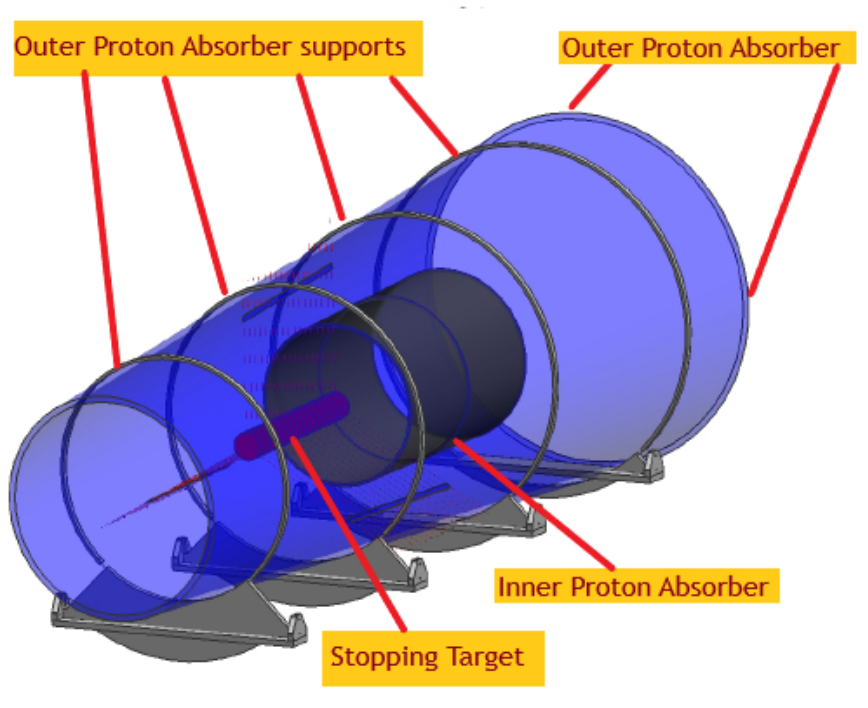
\includegraphics[width =0.5\textwidth]{figures/png/Screenshot_20240706_132949.png}
    \caption[The structure of the inner and outer proton absorber.]{The structure of the inner and outer proton absorber.}
    \label{fig:absorbersDS}
    \end{figure}




\section{Stopping Target}
The Mu2e ST, Figure \ref{fig:ST}, is 
composed of 37 annular aluminum foils of 75 mm of radius with a purity of 
above 99.99\% \cite{bobbb}. The foils are 100 $\mu$m thick to minimize energy losses of the CEs. This design 
narrows the reconstructed CE momentum distribution 
and separates it from the DIO electron momentum distribution. 
The disks have an internal hole of 21 mm of radius.
The annular design minimizes interactions with the beam electrons, reducing the radiation load by $\sim$30\%.

The central hole does not affect the target capacity to halt muons, 
which move in helical patterns. The space between each disk is
22.2 mm, bringing the total lenght of the ST to $\sim$80 cm.
Muons passing through the hole of an upstream foil will stop in a downstream layer. 
The design of the ST has been chosen by considering two 
conflicting physical requirements. Firstly, the target must be thick enough 
to stop a significant fraction of the muons, with the current version achieving 
an indicative stopping fraction of 30\%.

Secondly, the target must be thin 
enough to control the energy loss of the CEs, which is why 
the target has a segmented geometry.
\begin{figure}[!h]
    \centering
    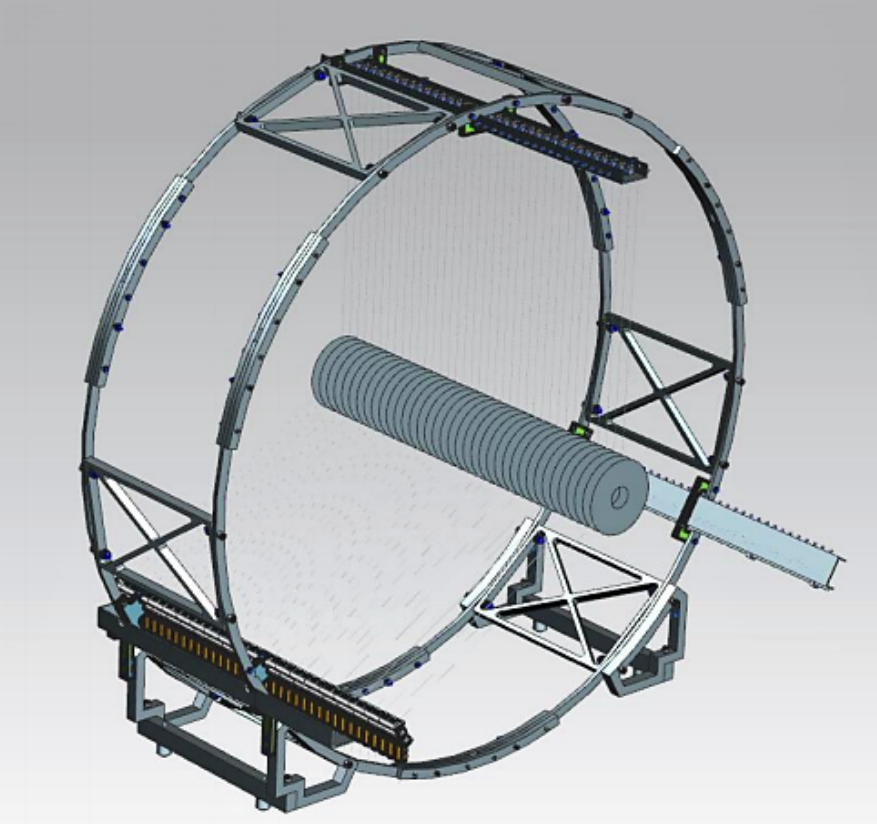
\includegraphics[width =0.5\textwidth]{figures/png/Screenshot_20240706_122723.png}
    \caption[The Stopping Target design.]{The ST design. 
    Each disk is supported by three cables not shown in the picture }
    \label{fig:ST}
\end{figure}

There are various factors to consider while selecting aluminum as the ST material. 
First, as described in Section \ref{backgrounds}, the aluminum 
target has a lower RMC background. Moreover, the muonic aluminium 
atom has a quite long lifetime, as shown in Figure \ref{fig:muonicatom}. 
The long lifetime allows separation between prompt backgrounds and a 
live window with a good decay rate. The muon DIO endpoint energy, 
further, depends on the type of nucleus, as shown in Figure \ref{fig:endpoint}. 
Aluminum has a high endpoint energy, so when muons are captured on other 
detector materials with a higher atomic number $Z$, they have lower 
endpoint energies and do not contribute to background. For these reasons, aluminum is a 
suitable ST material for muon-to-electron conversion searches.
Moreover, the branching ratio ($BR$) of the conversion varies 
depending on the ST material due to differences in atomic number 
($Z$) and mass number ($A$). By comparing $BR$s on different nuclei 
normalized to aluminum, it is possible to identify the dominating 
operator type, such as scalar ($S$), dipole ($D$), vector of 
transition charge radius type and vector of effective $Z$-penguin type, 
($V(\gamma)$) and ($V(Z)$) respectively. 
Despite challenges in separating prompt backgrounds from 
signals due to short lifetimes of muonic atoms, 
materials with higher $Z$ offer better model differentiation. 
If the Mu2e experiment observes conversion signals, a subsequent search 
could make use of titanium as the ST. A more detailed discussion can be 
found in \cite{PhysRevD.80.013002}, \cite{PhysRevD.76.059902} and 
\cite{abusalma2018expression}.


\begin{figure}[!h]
    \centering
    \begin{subfigure}[t]{0.5\textwidth}
        \centering
        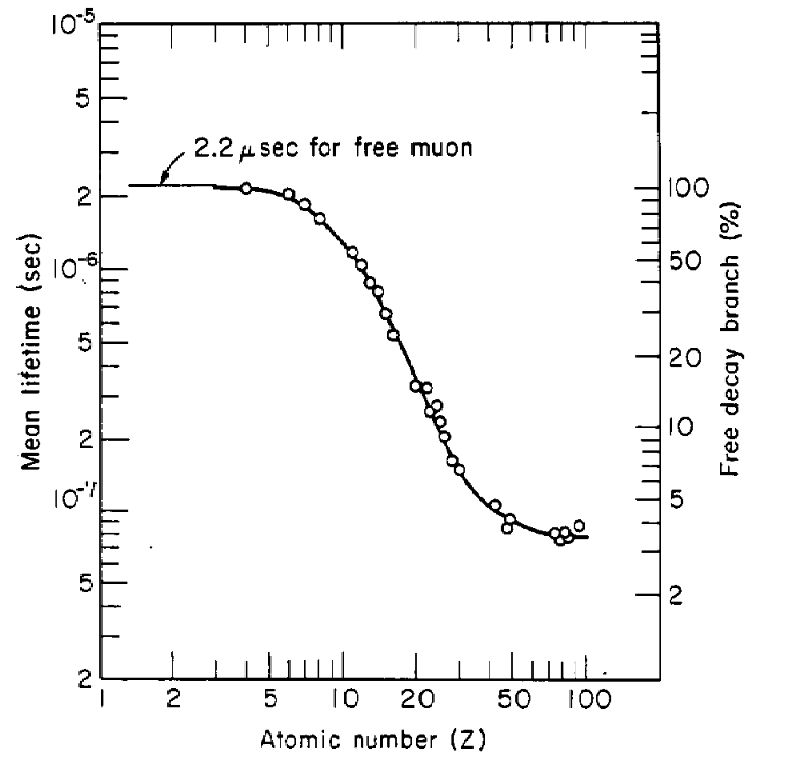
\includegraphics[width=0.85\textwidth]{figures/png/lifetime_mu_matter.png}
        \caption{}
        \label{fig:muonicatom}
    \end{subfigure}%
    ~ 
    \begin{subfigure}[t]{0.5\textwidth}
        \centering
        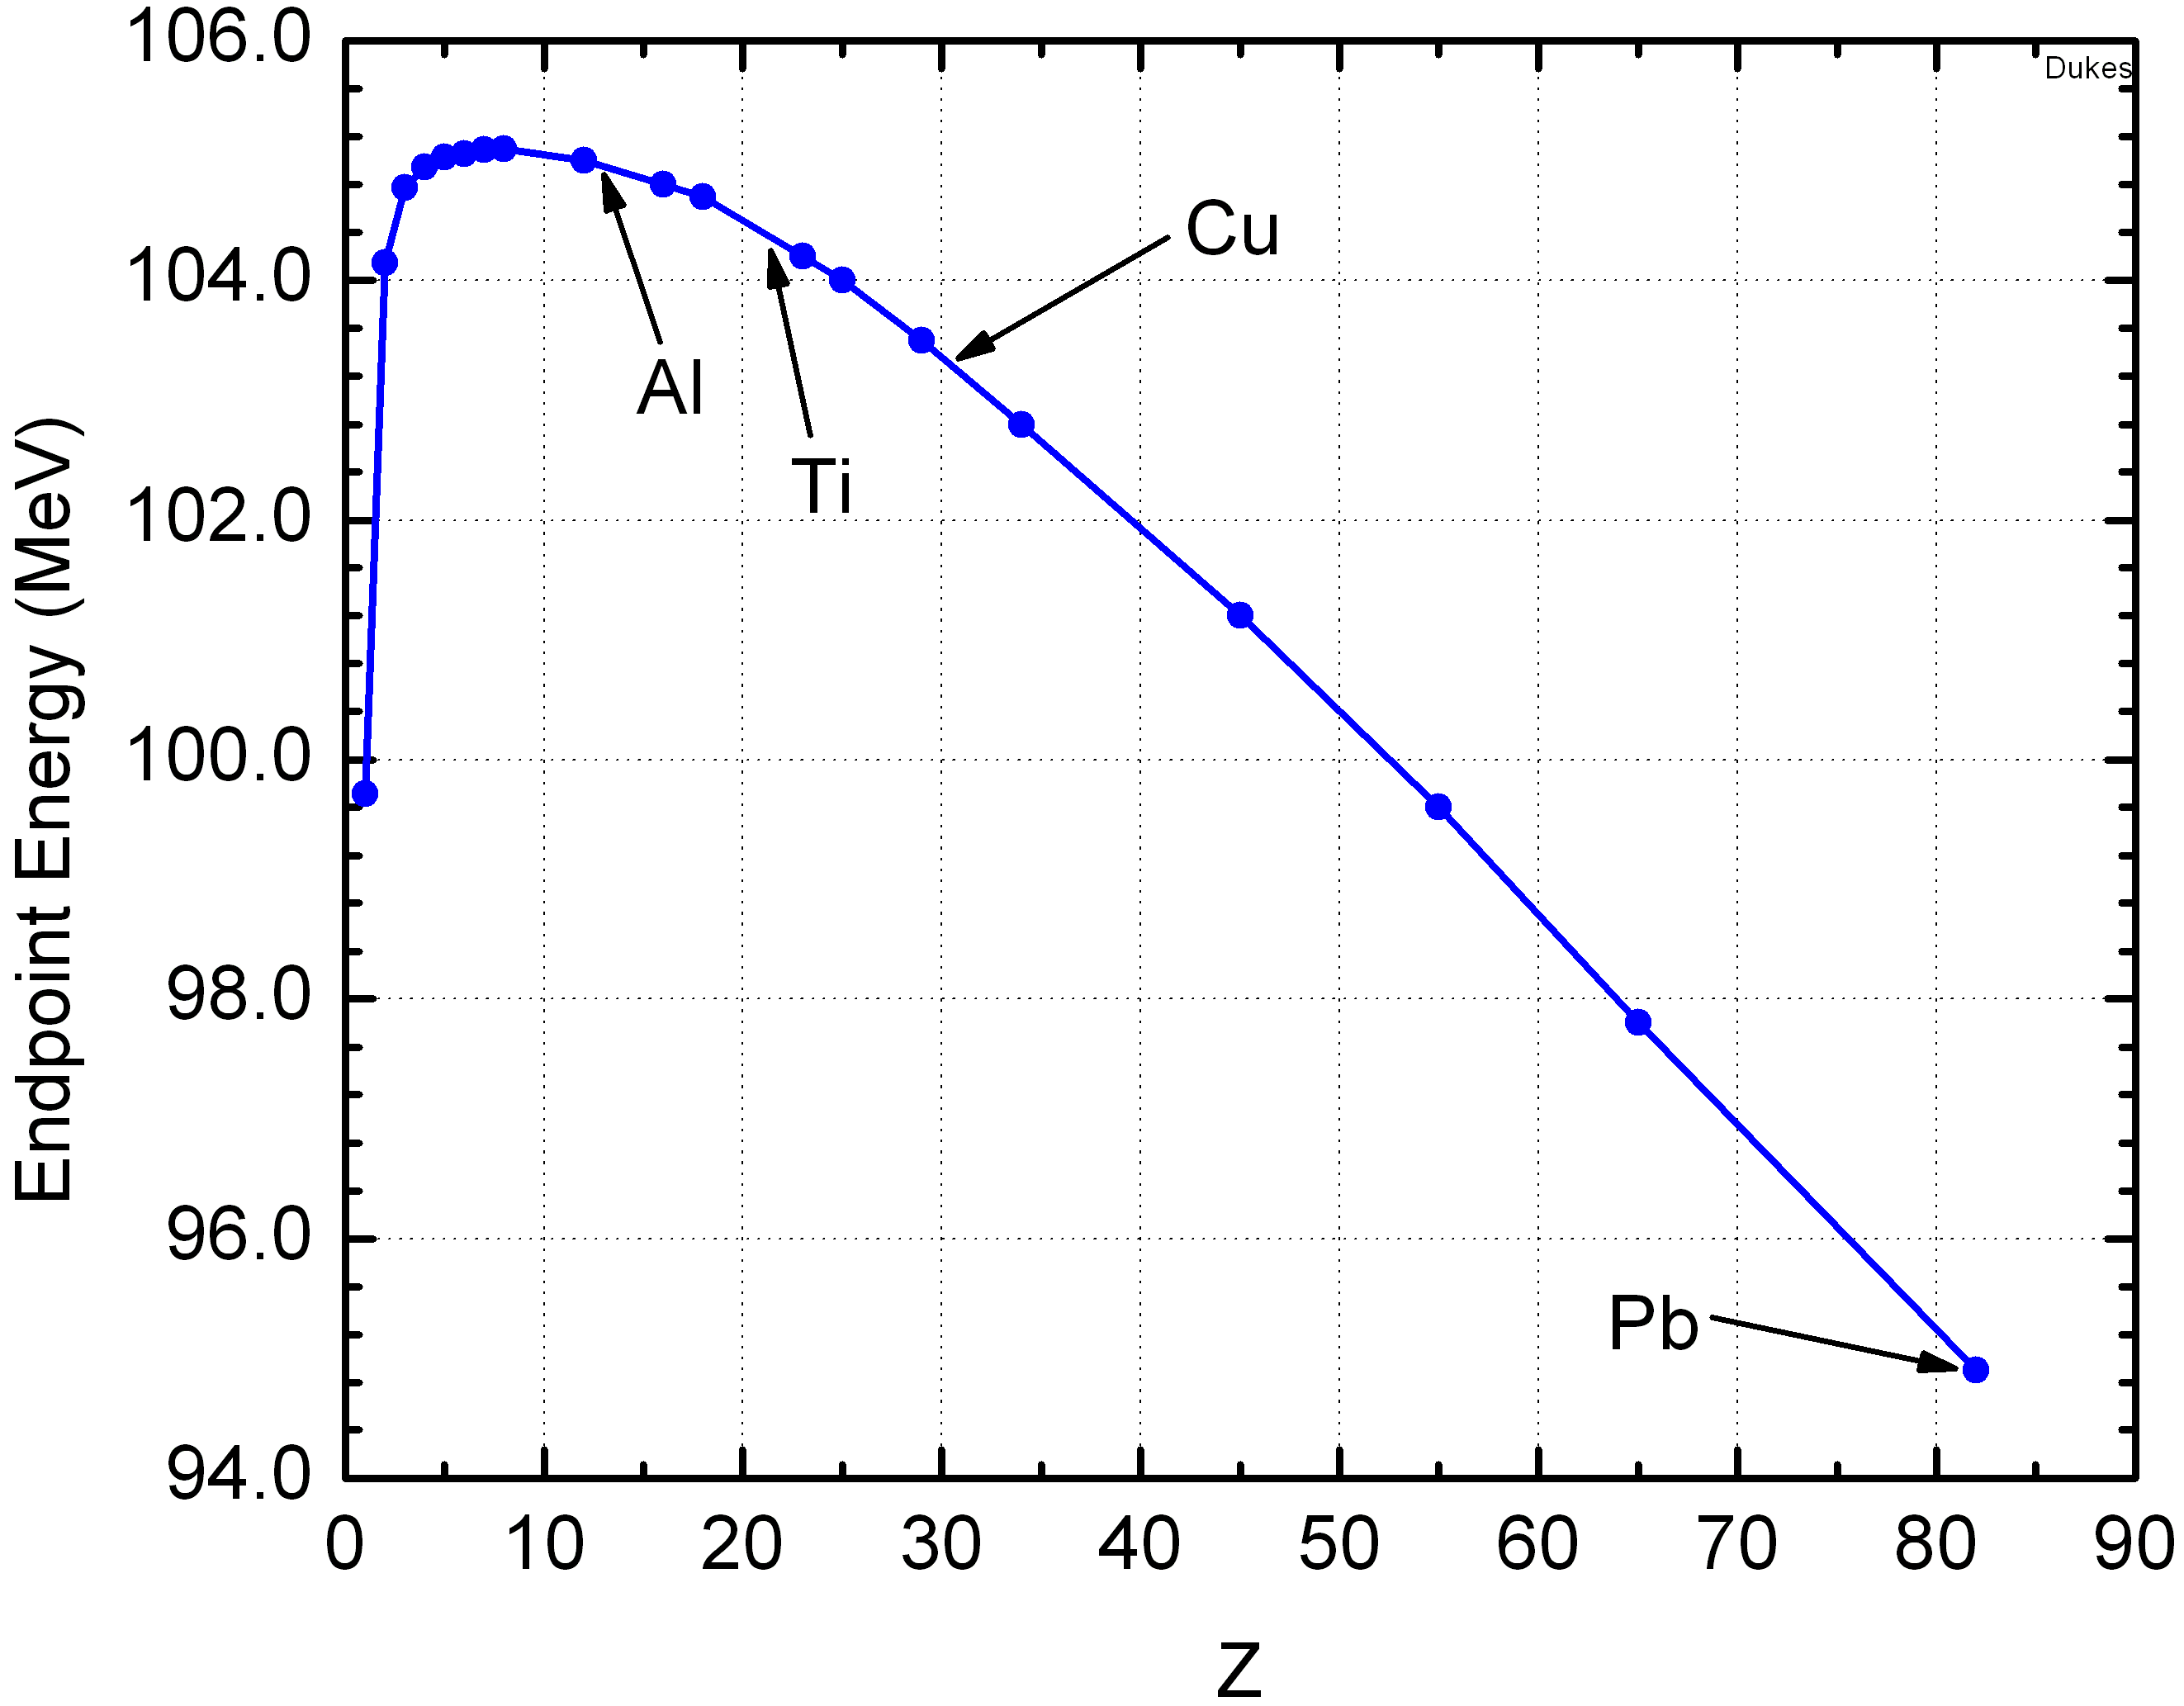
\includegraphics[width=0.85\textwidth]{figures/png/endopint.png}
        \caption{}
        \label{fig:endpoint}
    \end{subfigure}
   \caption[The muonic atom mean lifetime and muonic free decay fraction. The dependence 
   of the electron energy spectrum endpoint
   on the DIO.]{(a) The dependence of the mean lifetime and free decay fraction 
   of the muonic $1s$ state on the atomic number of the nucleus to which 
   the negative muon is bound \cite{TYamazaki_1975}, and (b) 
   the dependence of the electron 
   energy spectrum endpoint on the DIO \cite{dukes}.}
    \label{fig:2imins}
  \end{figure}
\section{The Mu2e detectors}
Mu2e makes use of a set of complementary detectors to 
measure particles momentum and energy. These detectors 
are annular and situated within a solenoidal magnetic field of 
approximately 1 T along the $z$-axis, which aligns with 
the direction of the muon beam. This distinctive geometry 
is highly effective in reducing background, as it allows 
the passage of particles produced during muon capture, 
remnant beam, and electrons from the initial proton collision to the beam dump without striking
the detector elements, that otherwise would cause excessive instantaneous detector 
occupancy and accumulated radiation damage. 
Most decay muons are tipically too low momentum 
to exit the central region, preventing them from reaching the detector elements. 
As a result, the number of detector hits is kept at a manageable level. 
Due to acceptance limitations for particles originating from the ST, 
only particles with a momentum higher than 80 MeV/c can be reconstructed.
The Mu2e detection system comprises a straw tracker, followed by a 
calorimeter and a STM, all enclosed within the CRV.


\subsection{The straw tracker}\label{trackersec}
The Mu2e straw tracker is placed inside the DS downstream from 
the ST in a 1 T uniform magnetic field. The tracker is one of the most 
important Mu2e detectors: it must provide very good momentum resolution to 
disentangle the monochromatic CE signal from the background. 
Since the shape of the DIO spectrum near the endpoint decreases as 
$(E_{\mu e} -E_e)^5$, the corresponding background increases very quickly as the resolution
degrades. To achieve the desired DIO suppression, the required momentum resolution should be below 1 MeV/c.  
Figure \ref{fig:trkres} shows the expected momentum resolution as determined 
from a full GEANT4 simulation of the detector, Front-End Electronics (FEE), and the DAQ.
It is fundamental to have a thorough understanding of the tails of the momentum resolution. 
The right tail could push low-energy DIO electrons into the CE signal window. 
On the other hand, the left tail, which is primarily due to energy losses in the ST, 
in the IPA, in the OPA, and in the tracker itself, could 
push CEs below the signal window in the region dominated by DIOs 
thus reducing the signal efficiency.
\begin{figure}[!h]
    \centering
    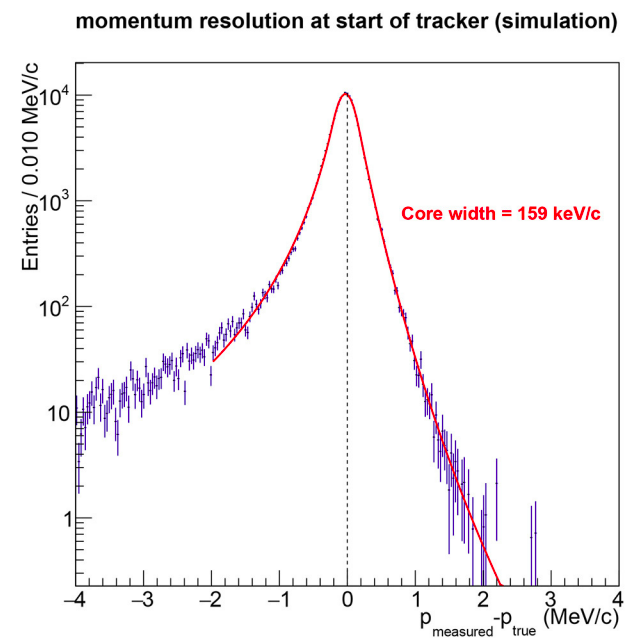
\includegraphics[width =0.5\textwidth]{figures/png/Screenshot_20240330_104830.png}
    \caption[The momentum resolution of the straw tracker.]{Momentum resolution of the straw tracker as determined for 
    a sample of Monte Carlo CEs \cite{bobbb}.}
    \label{fig:trkres}
    \end{figure} 
To minimise the probability of scattering and the energy loss of the CE, 
the volume inside the DS is evacuated to $10^{-4}$ Torr. 
The Mu2e collaboration has selected the straw-tube 
technology \cite{bobbb} for its tracker, driven by the need for 
a detector with high core resolution, minimal high-side tails, 
and low energy loss. This choice led to straw tubes, which 
offer a combination of low mass, rapid drift times, good spatial 
resolution and they are in wide use in particle physics. 

The detector has an annular shape with an active region covered by straws only between the 
internal radius of 380 mm and the external radius of 700 mm.  

Chapter \ref{chaptertrk} will provide a more detailed description of the entire detector, 
including the mechanical structure, the FEE and 
DAQ system.
\subsubsection{Momentum scale calibration}
One of the most challenging aspects of the Mu2e experiment is achieving the 
required momentum resolution to distinguish the CE electron from the background.

Mu2e requires at least one source of high-energy calibration electrons or 
positrons to independently measure the absolute momentum scale of the tracker. 
The momentum scale calibration relies on accurately reconstructing the 
$\pi^+ \rightarrow e^+ \nu_e$ peak ($BR\sim 1.23 \times 10^{-4}$), with its success critically dependent on the 
suppression of $\mu^+ \rightarrow e^+ \nu_e \bar{\nu}_\mu$ decays in flight (DIF). 
Several approaches have been explored, with the most promising ones being:

\begin{enumerate}
    \item Special run with adjusted TS collimators: operating with 
    reversed TS collimators and a reduced DS field 
    (70\% of the nominal value), this setup is designed to capture the 
    leptonic decay ($\pi^+ \rightarrow e^+ \nu_e$) of stopping $\pi^+$ in the nominal ST;
    
    \item Low intensity run with reduced DS magnetic field: 
    running at low intensity and a further reduced DS field 
    (50\% of the nominal value), 
    this approach aims to gather high-statistics data to accurately fit 
    the Michel edge of the DIO momentum distribution.
\end{enumerate}

Several important considerations include:

\begin{itemize}
    \item Early time measurement: to reconstruct the $\pi^+ \rightarrow e^+ \nu_e$ decays, 
    measurements must be performed at early times, approximately 
    $T \sim 300$ ns. This necessitates operating at a reduced proton 
    beam intensity to mitigate the pileup;
    
    \item Special instrumentation requirement: to minimize 
      the background from muon decays in flight, a beam degrader
      in the DS is needed.
\end{itemize}

The momentum scale calibration described involves two key measurements: 
\begin{enumerate}
    \item The edge of the positron momentum spectrum 
    from $\mu^+ \rightarrow e^+ \nu_e \bar{\nu}_\mu$ decays 
    at $B = 0.5$ T;
    \item The $\pi^+ \rightarrow e^+ \nu_e$ peak at $B = 0.7$ T.
\end{enumerate}

Each of these measurements determines the momentum scale at their respective 
magnetic field values. By combining these measurements, we can extrapolate the 
momentum scale to the nominal magnetic field, $B = 1.0$ T. This concept is illustrated in Figure \ref{fig:momscale}.

\begin{figure}[!h]
\centering
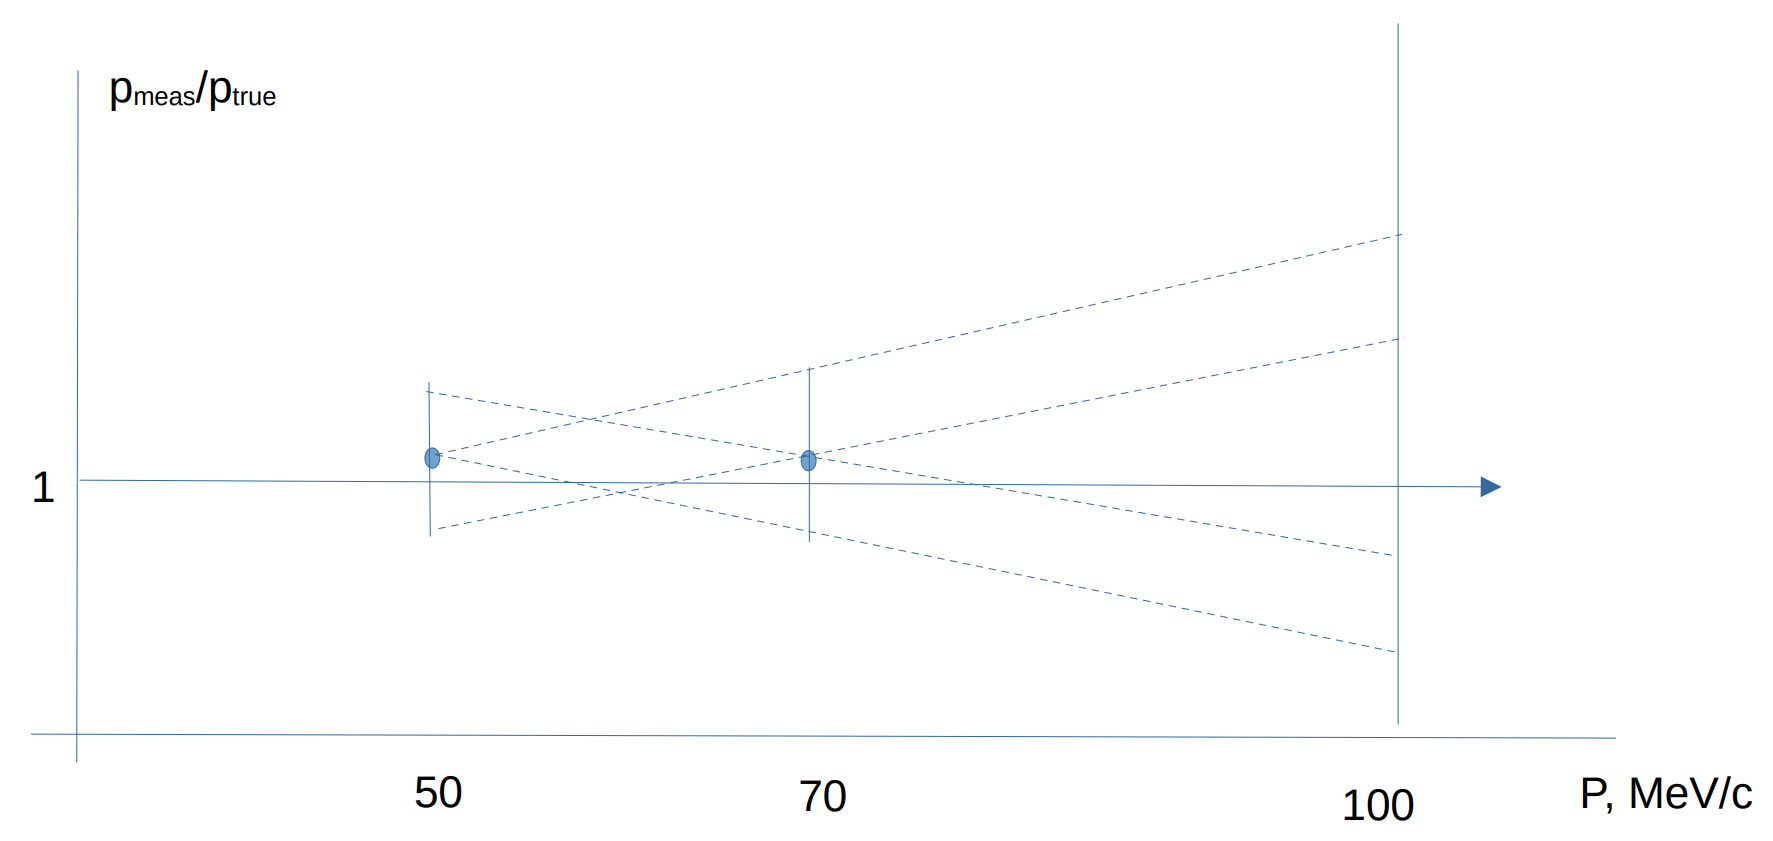
\includegraphics[width=0.7\textwidth]{figures/png/Screenshot_20240909_140555.png}
\caption[The momentum calibration scheme.]{Illustration of the momentum calibration scheme.}
\label{fig:momscale}
\end{figure}

The calibration scheme assumes that the magnetic field is initially set based 
on readings from an NMR probe.

\subsection{The electromagnetic calorimeter}\label{calorimeter}
The Mu2e electromagnetic calorimeter serves multiple purposes \cite{em4}:
\begin{itemize}
    \item the measurement of the energy deposited in the calorimeter 
    allows to separate electrons and muons of the same momentum. 
    The energy-to-momentum ratio ($E/p$) will be used for particle 
    identification and to suppress the background due to cosmic muons;
  \item the calorimeter information 
    helps improving the pattern recognition and 
    the quality of the track reconstruction;
    \item it provides independent triggers from the track-based triggers \cite{em6}. 
\end{itemize} 
For these purposes, the calorimeter needs to fulfill the following physical requirements:
\begin{itemize}
    \item an energy resolution better than $\sigma_E/E \sim$10\% allows
     to reach a rejection factor at the level of 200 between CE
    and the $\sim$ 40 MeV energy deposit from 105 MeV/c cosmic ray muons mimicking the signal;
    \item a timing resolution better than 500 ps ensures that
    the energy depositions in the calorimeter are in time with
    the CEs reconstructed by the tracker and
    also improves the PID;
    \item a position resolution of $\sim$6 mm allows 
    to match the position of the energy deposit with the 
    extrapolated trajectory of a reconstructed track;
    \item it should perform a fast enough 
      response in order to handle the experimental high rate ($\tau < 40$ ns);
    \item a temperature and gain stability within $\pm$0.5\% 
    are required not to deteriorate the energy resolution;
    \item it must be capable of operating in 
    a magnetic field of 1 T, a pressure of \(10^{-4}\) torr, a 
    neutron flux equivalent to \(10^{12}\) n/cm\(^2\)/year, 
    and in a high radiation environment (exposures up to 15 krad/year);
    \item reliability and redundancy are needed to operate in vacuum for one
    year without any interruptions.
\end{itemize}


The calorimeter disks are being assembled at Fermilab's SiDet facility, as shown in Figure 
\ref{fig:calostatus}. The components will be described in the next sections.

\begin{figure}[!h]
    \centering
    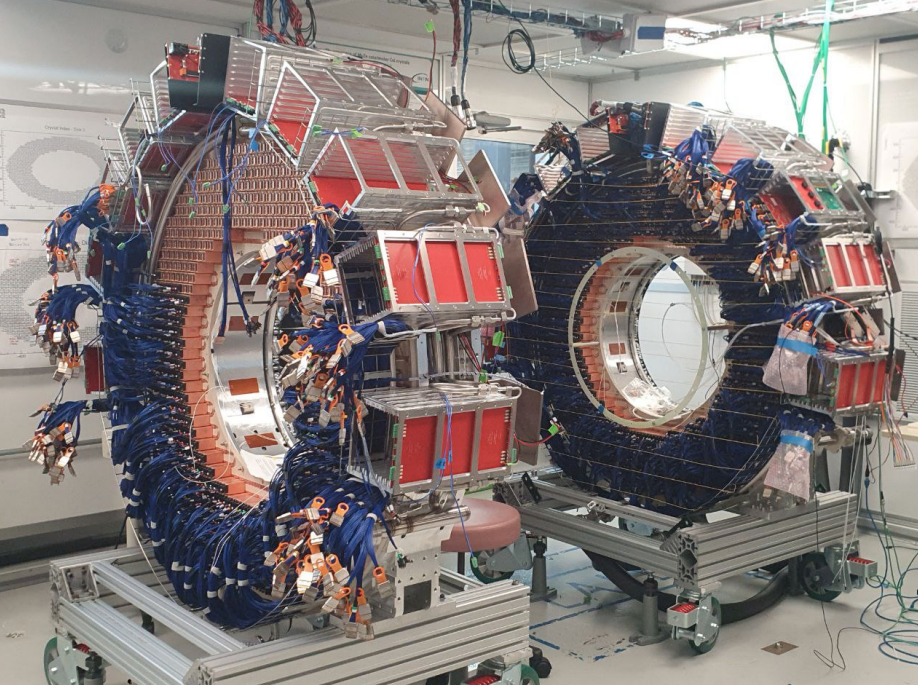
\includegraphics[width =0.6\textwidth]{figures/png/Screenshot_20240706_151533.png}
    \caption[The Mu2e calorimeter disks.]{Mu2e calorimeter disks being assembled at the Fermilab SiDet facility.}
    \label{fig:calostatus}
\end{figure}

\subsubsection{The calorimeter mechanical structure}
The calorimeter is located in the DS downstream of the tracker (Figure \ref{fig:DS})
It consists of two annular disks, with an internal radius of 35 cm and 
an external radius of 66 cm, located at a relative distance of 70 cm (Figure \ref{fig:calo1}).
The separation was chosen to match half of the distance between two periods of the helical trajectory 
of a typical 105 MeV CE. This maximises the detection probability of CEs: electrons which pass through the hole of the first disk will be detector by the second one \cite{em7}. 


The calorimeter mechanical structure was designed to support the layout of the crystals 
by piling them up in a self-standing array organized in consecutive staggered rows. 
Each crystal array is supported by two coaxial cylinders. The inner cylinder must be 
as thin and light as possible in order to minimize the passive material in the 
region where spiraling background electrons are concentrated. The outer cylinder 
is as robust as required to support the load of the crystals (700 kg). Each disk 
has two cover plates. The plate facing the beam is made of carbon fiber to minimize 
the degradation of the electron energy, while the back plate should also be robust 
to support the SiPMs, the FEE and the SiPM cooling lines and it 
is therefore made of Polyether ether ketone (PEEK). The crystal arrangement is 
self-supporting, with the load carried primarily by the outer ring. 
The heat generated by SiPMs, FEE and read out electronics 
must be removed within temperature values acceptable for the correct operation 
of each device. Furthermore, the difficult access to components requires a 
cooling system free of fault and maintenance needs for at least one year. 
The cooling system has to maintain SiPM temperature at approximately -10°C to 
minimize the dark current: this is obtained by circulating a refrigerating fluid at approximately  -15°C.


\begin{figure}[!h]
    \centering
    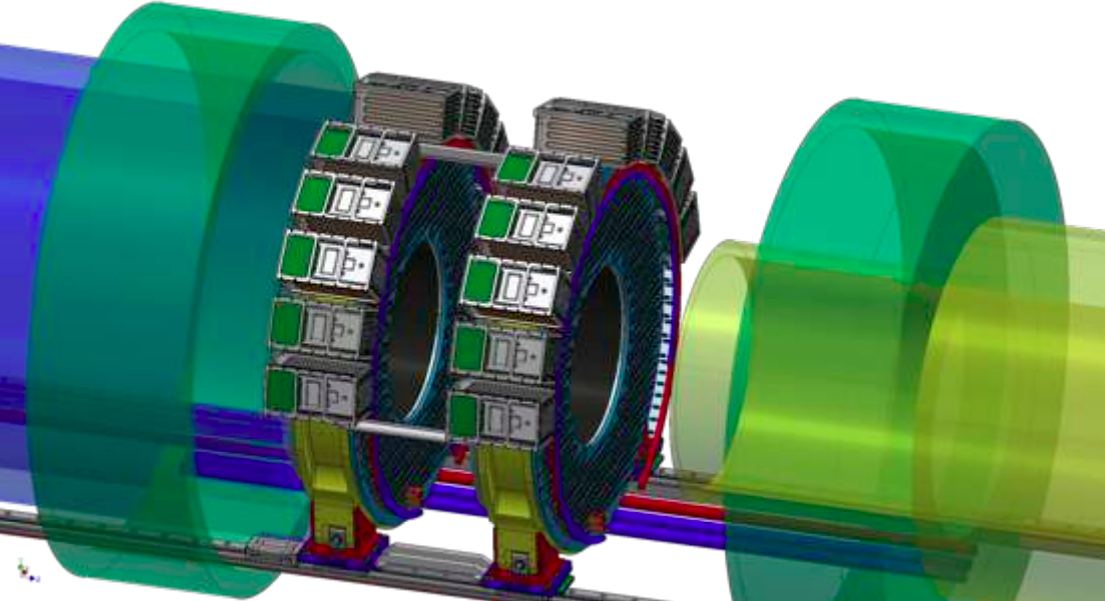
\includegraphics[width =0.6\textwidth]{figures/png/Screenshot_20240322_122050.png}
    \caption[CAD representation of the calorimeter disks.]{Calorimeter disks installed in the Mu2e experimental area (CAD representation) \cite{em7}.}
    \label{fig:calo1}
\end{figure}



\subsubsection{The undoped Cesium Iodide crystals}
Each calorimeter disk is filled with 674 undoped cesium 
iodide (CsI) crystals \cite{em6}, wrapped in a 150 $\mu$m Tyvek foil. 
Undoped CsI represents the best compromise between cost, 
reliability, performance and radiation hardness, providing 
a fast emission time and a sufficiently high light yield. Pure 
CsI has a wavelength peak emission at 310 nm, a scintillation 
time of 20 ns, and a light yield of about 2000 photons/MeV. 
Figure \ref{fig:calo2} (top right) shows some CsI crystals: 
the dimensions are 34$\times$34 200 mm$^3$. The crystal length 
is approximately 10$X_0$ which is sufficient to contain the 105 
MeV CE shower since the average incident angle 
is 50°. Undoped CsI crystals also have the radiation hardness 
adequate for the Mu2e operational conditions. 




\begin{figure}[!h]
    \centering
    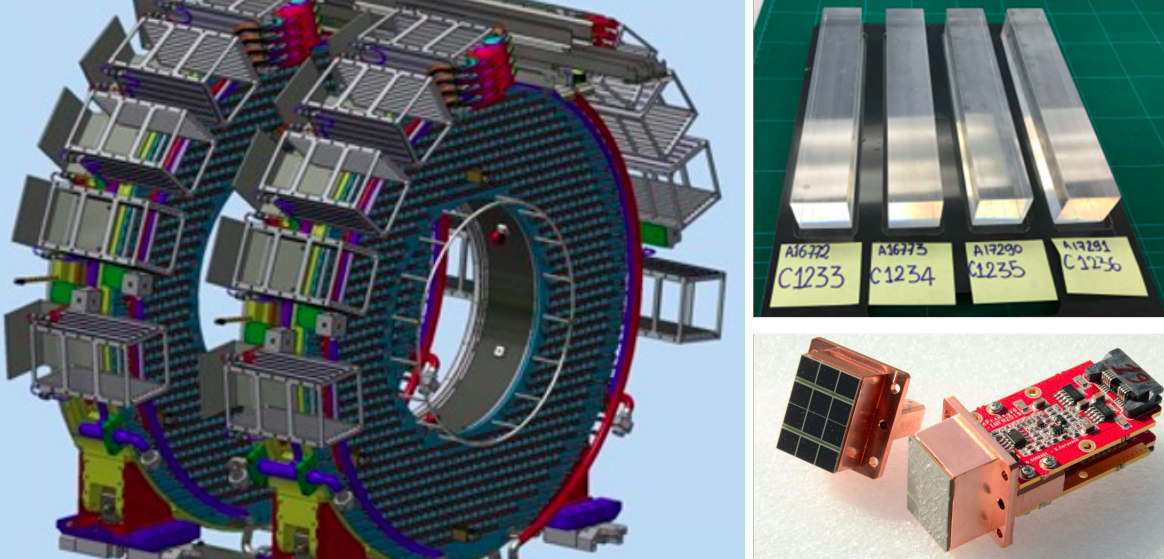
\includegraphics[width =0.7\textwidth]{figures/png/Screenshot_20240322_121000.png}
    \caption[The calorimeter components.]{(Left): Schematic CAD representation of the two calorimeter disks. (Top right): 
    cesium iodided crystal used in the calorimeter. (Botto, right): Two SiPM arrays 
    glued onto the copper holder (left) and one fully assembled readout unit made of two 
    SiPM arrays and two Front-End boards mounted on the copper holder (right) \cite{em4}.}
    \label{fig:calo2}
\end{figure}


\subsubsection{The calorimeter readout chain}
The readout of the calorimeter is performed through a chain of components: Silicon PhotoMultipliers (SiPM), 
FEE, Mezzanine board and Digitizer board. In the following, 
a brief description of each component will be provided.
\paragraph{Silicon PhotoMultipliers (SiPM)}
Since the calorimeter will operate in a 1 T magnetic field, SiPMs were chosen over PMTs (Figure \ref{fig:sipmcell}) \cite{em1}. 
To well match the scintillation emission of 310 nm to the SiPM photon detection efficiency, 
UV extended Hamamatsu SiPMs with a front window made of a silicon resin were selected. Each SiPM is composed of a
2 $\times$ 3 array array of individual 6 mm $\times$ 6 mm cells.
The array can be seen as the parallel of two series of 3 cells, that 
are powered by the same source. The mixed configuration is motivated by 
two competing requirements: a parallel connection has greater capacitance and a higher response time 
but requiring a lower bias voltage, whereas 
a series connection has the opposite characteristics. 
To improve reliability, light collection efficiency and resolution, each single 
crystal is readout by two custom SiPMs arrays.
Magnetic field resistance was the factor in choosing between SiPMs and PMTs.
The good efficiency of the SiPMs allows to collect approximately 20 p.e./MeV per SiPM.
To operate in vacuum, minimise outgassing contributions, reduce 
thermal coupling between crystals and FEE, the crystal-SiPM 
coupling is done without any optical grease and a 2 mm air gap is mantained 
between the crystal and the readout sensor.

Since the main scintillation component has a wavelength of 315 nm to match the SiPM
photon detection efficiency as a function of wavelength, each crystal is coupled with a readout 
module consisting of two ultraviolet (UV)-extended SiPM arrays
and the corresponding analog FEE boards, as illustrated in Figure 
\ref{fig:calo2} (bottom right) \cite{em5}, \cite{em2} and \cite{em3}. 
As shown in Figure \ref{fig:calo3}, each board is positioned within the electronic 
crates that surround the calorimeter disks.
\begin{figure}[!h]
        \centering
        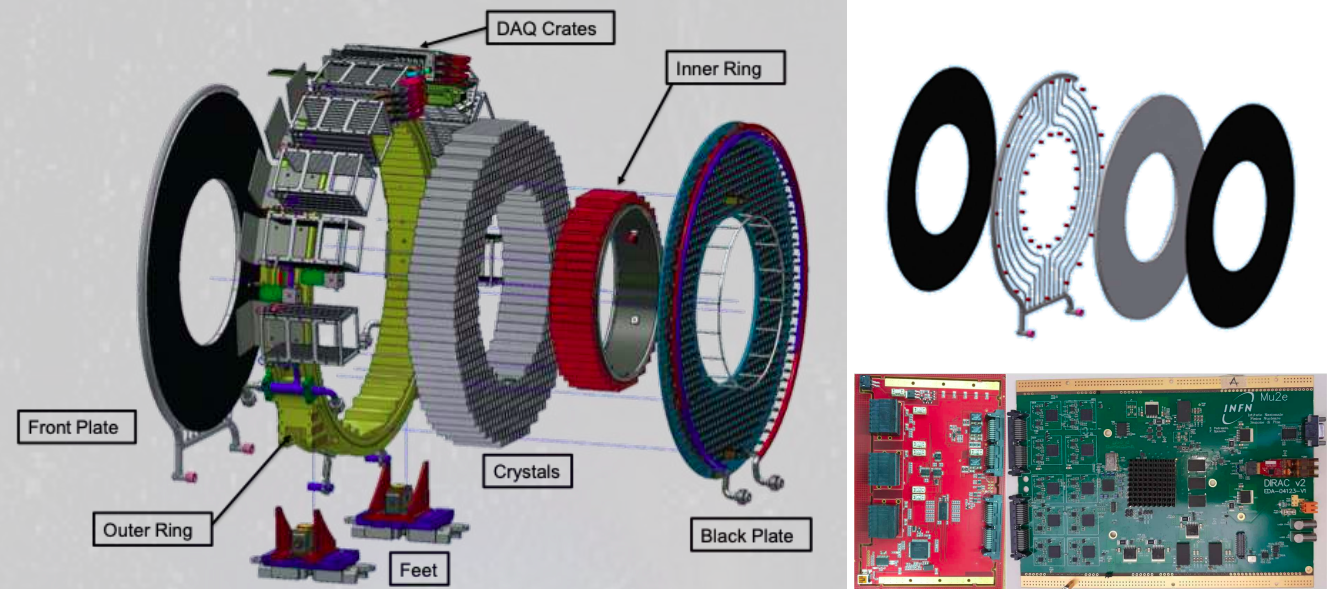
\includegraphics[width =0.8\textwidth]{figures/png/Screenshot_20240322_121017.png}
        \caption[The breakout of calorimeter mechanical components.]{Left: the breakout of calorimeter mechanical components. Top right: the breakdown of front
        panel plate. Bottom right: the Mezzanine and DiRAC boards \cite{em4}.}
        \label{fig:calo3}
        \end{figure}


\begin{figure}[!h]
    \centering
    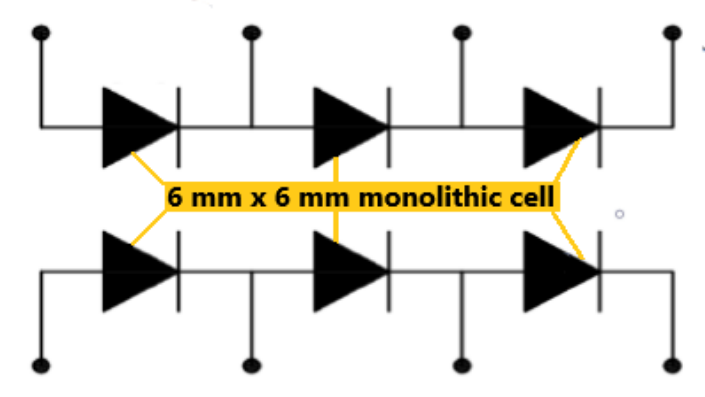
\includegraphics[width =0.6\textwidth]{figures/png/Screenshot_20240706_141625.png}
    \caption[The design of SiPM cells.]{The design of a 2$\times$3 array of SiPM cells.}
    \label{fig:sipmcell}
\end{figure}
\paragraph{The Front-End electronics}
Each SiPM is read by one Front-End board directly linked to the pins on the 
back of the SiPMs and, via cable, to the Mezzanine board (Figure \ref{fig:connectiontomezzanine}). 
The Front-End board provides signal preamplification and shaping, local linear 
regulation of the SiPM bias voltage, and monitoring of the SiPM current and temperature. 
The two Front-End boards connected to the two SiPMs reading the same CsI 
crystal are housed in a copper holder (Figure \ref{fig:holder}), which 
serves as a mechanical support and ensures SiPM cooling. 
An enternal Faraday cage reduces the noise. The holder also holds 
an optical fiber used to pulse the crystal with a laser light to 
calibrate the energy and time response.
\begin{figure}[!h]
    \centering
    \begin{subfigure}[t]{0.5\textwidth}
        \centering
        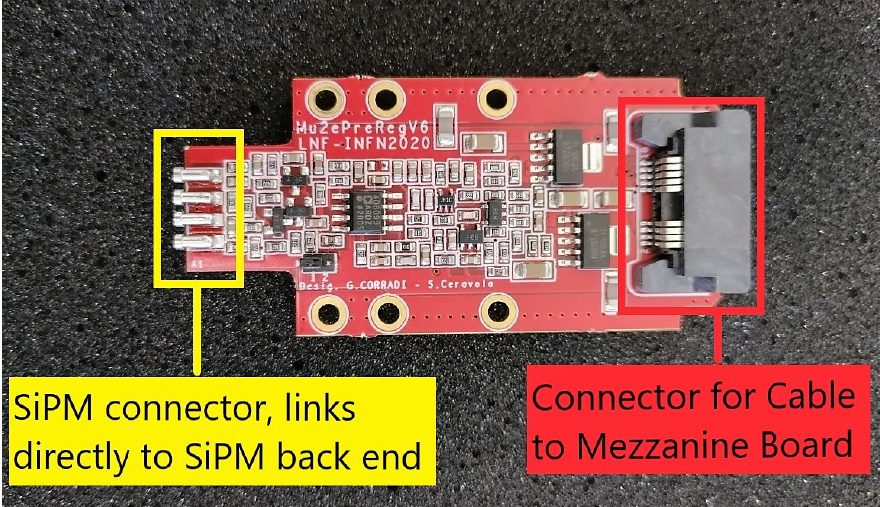
\includegraphics[width=0.85\textwidth]{figures/png/Screenshot_20240706_143204.png}
        \caption{}
        \label{fig:connectiontomezzanine}
    \end{subfigure}%
    ~ 
    \begin{subfigure}[t]{0.5\textwidth}
        \centering
        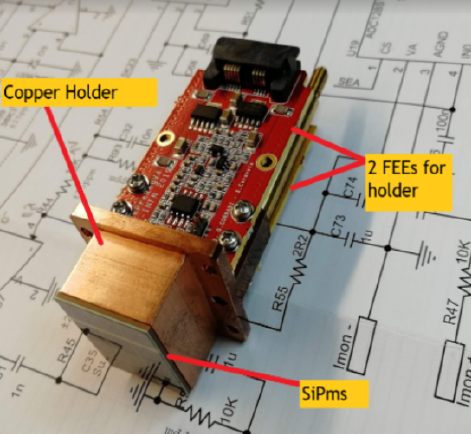
\includegraphics[width=0.85\textwidth]{figures/png/Screenshot_20240706_143517.png}
        \caption{}
        \label{fig:holder}
    \end{subfigure}
   \caption[The calorimeter FEE board.]{(a): The FEE board, with its connectors to SiPMs 
   back and to the cable coming from Mezzanine. 
   (b): The assembled FEE holder.}
    \label{fig:calooo}
  \end{figure}


\paragraph{The Mezzanine board}
The Mezzanine Board serves as the interface between 20 different 
Front-End boards and one Digitizer (Figure \ref{fig:mezzanine}) 
The Mezzanine sets all FEE parameters (such as High Voltage (HV)) and 
monitors all Front-End boards and SiPM parameters (such as HV, temperature, and current). 
It also provides low voltage to the Front-End boards. The HV of each SiPM can be 
independently set. These tasks are performed by an ARM processor located on the 
Mezzanine board. The cables chosen to link the Front-End boards to the 
Mezzanine board must be radiation-resistant, shielded, and have low outgassing. 
\begin{figure}[!h]
    \centering
    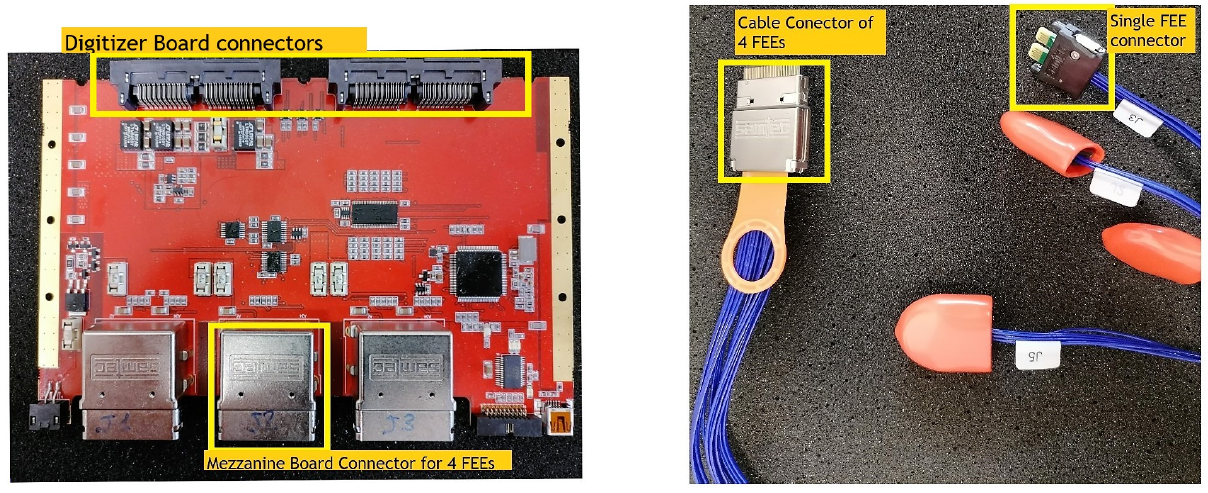
\includegraphics[width =0.8\textwidth]{figures/png/Screenshot_20240706_144234.png}
    \caption[The calorimeter Mezzanine Board and FEE.]{Left: The Mezzanine Board with connectors highlighted. 
    Right: The Cable linking 4 FEEs to one Mezzanine.}
    \label{fig:mezzanine}
\end{figure}



\paragraph{The digitizer Board}
The Digitizer Readout Controller (DiRAC) digitizes the SiPM 
signals received from the Mezzanine Board and manages data 
transmission to the experiment's DAQ system. Zero suppressed 
data are sent from the DiRAC board to the DAQ via optical fibers. 
A sampling rate of 200 MHz (one sample every 5 ns) and a 12-bit resolution 
satisfy the calorimeter requirements. The two SiPMs which read the same 
crystal are always connected to different DiRAC boards hosted in separate 
crates to prevent a complete loss of a crystal 
in an event of a single crate fault.

\paragraph{The crate}
The Mezzanine and DiRAC boards reside in crates.
Each crate contains up to eight Mezzanine 
and DiRAC boards and provides cooling to the boards via a network of cooling lines grooved in the crate walls.
The thermal contact between the electronics components on the Mezzanine and the DIRAC
and the crate walls is ensured by a copper plate covering the entire board.
\subsubsection{Module-0 prototype}
To validate the chosen design before commencing the mass production of 
the calorimeter components, a large-scale prototype was constructed and 
tested with an electron beam at the Beam Test Facility of the National 
Laboratories of Frascati. The Module-0 consists of 52 undoped CsI crystals, 
read by 102 SiPMs connected to FEE boards. Its mechanics was designed

to closely resemble the final calorimeter, allowing for the testing 
of the assembly procedures and cooling.
The energy and time resolution are
shown in Figure \ref{fig:calores} \cite{bobbb} and \cite{calo95}.
\begin{figure}[!h]
    \centering
    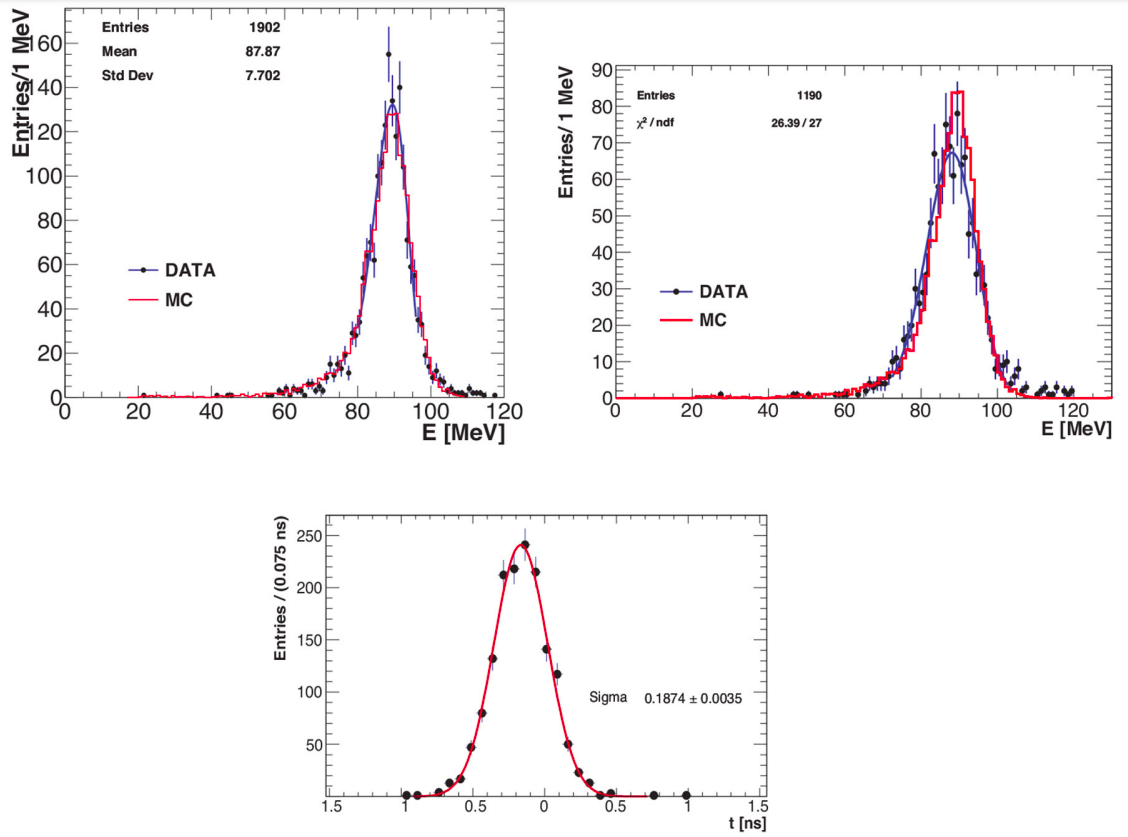
\includegraphics[width =0.8\textwidth]{figures/png/Screenshot_20240330_105520.png}
    \caption[The energy and time resolution of the calorimeter Module-0.]{The 
    energy and time resolution of the Module-0 for the Mu2e 
    calorimeter for electrons at the conversion energy. (Top left) The resolution 
    for electrons striking the array at normal incidence. (Top right) 
    Resolution for electrons striking the array at 50° with respect to the 
    face. (Bottom) The time resolution. All measurements are compared with 
    simulations (red line) \cite{bobbb} and \cite{calo95}.}
    \label{fig:calores}
\end{figure}
\subsection{The Cosmic Ray Veto}\label{CRV}
As reported in the Section \ref{backgrounds}, the expected Mu2e 
cosmic background is at a level of 1 signal-like event per day. 
To minimize the backgrounds, Mu2e exploits a combination of passive shielding and an active 
veto system named CRV. Figure \ref{fig:crv} shows a 
schematic representation of 
the CRV covering the region of the DS and half of the Transport Solenoid 
almost entirely (there is no veto on the floor at the bottom), for a total detector area
of 327 m$^2$.
The CRV modules are manufactured from plastic scintillator extrusions. 
In different regions of the detector the extrusions may have different lenghts, 
but they all have the same cross-sectional area of $5 \times 2$ cm$^2$.
The extrusions 
are coated with Titanium dioxide to improve internal reflections and thus, the light yield. 
Two grooves are extruded inside the scintillator bar throughout its length to contain two 
1.4 mm diameter wavelength shifting fibers. The fibers transport light to the extrusion 
ends where each fiber is instrumented with a $2 \times 2$ mm$^2$ SiPM at each end. Figure \ref{fig:crvmodule} 
shows the cross-section of a CRV module. Each module is made of four overlapping staggered layers 
of plastic scintillator counters to reduce the effects of gaps. The 
layers are separated by 10 mm aluminium plates used as absorbers. 
When three of the four layers of the CRV are activated, an offline veto window is opened.
A conversion-like event observed during this time window is assumed to be produced by a cosmic-ray muon
and will be disregarded. 
The estimated total dead time is $\sim$5\%.
Based on the simulation, the required CRV veto efficiency is 99.99\% within the detector fiducial.

\begin{figure}[!h]
\centering
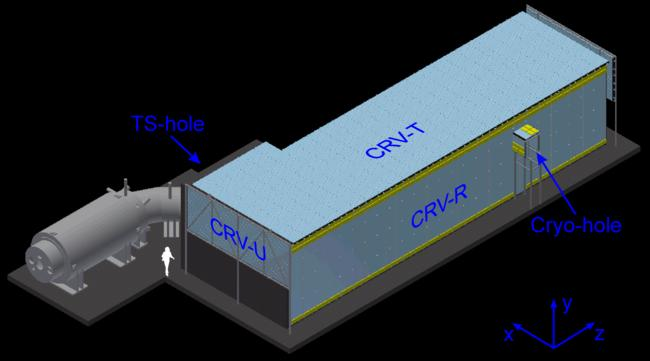
\includegraphics[width =0.65\textwidth]{figures/jpg/Crv_downstream.jpg}
\caption[The CRV features and components.]{The CRV covers the DS entirely and half 
of the Transport Solenoid. It is made of several sectors, including the top 
(CRV-T), the right (CRV-R), the left (CRV-L), the upstream (CRV-U), the downstream 
(CRV-D), and the hole where the Transport Solenoid enters the enclosure (TS-hole) \cite{bartoszek2015mu2e}.}
\label{fig:crv}
\end{figure}

\begin{figure}[!h]
\centering
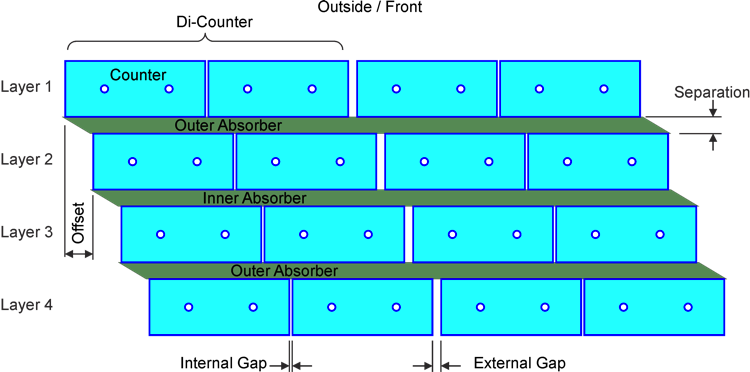
\includegraphics[width =0.65\textwidth]{figures/png/Crv_module_geometry.png}
\caption[The cross-section of a CRV module.]{Cross-section of a CRV module, including geometry and nomenclature. 
There are internal gaps between counters in a di-counter \cite{Giovannella_2020}.}
\label{fig:crvmodule}
\end{figure}
\subsection{The Muon Beam Stop and the Stopping Target Monitor}
A Muon Beam Stop (MBS) is installed at the downstream end of the DS to 
absorb muons that are not stopped in the ST, shown in Figure \ref{fig:stm}. 
The MBS has been designed to limit the effects of muon decays and captures. 
The magnetic field gradient prevents the majority of the low-energy charged 
particles created in the MBS from moving upstream towards the detectors.  
The MBS is made of high-$Z$ minerals and polyethylene. Muons have an extremely short lifetime in 
high-$Z$ materials, as shown in Figure \ref{fig:muonicatom}, which minimizes the effects of muon 
decays and captures much earlier than the Mu2e live window starting at 640 ns. Moreover, polyethylene 
absorbs protons and neutrons emitted by the excited nuclei during muon captures.  

The STM is placed downstream from the MBS, as shown in Figure \ref{fig:stm}, 
to measure the number of muons stopped on the ST.

\begin{figure}[!h]
    \centering
    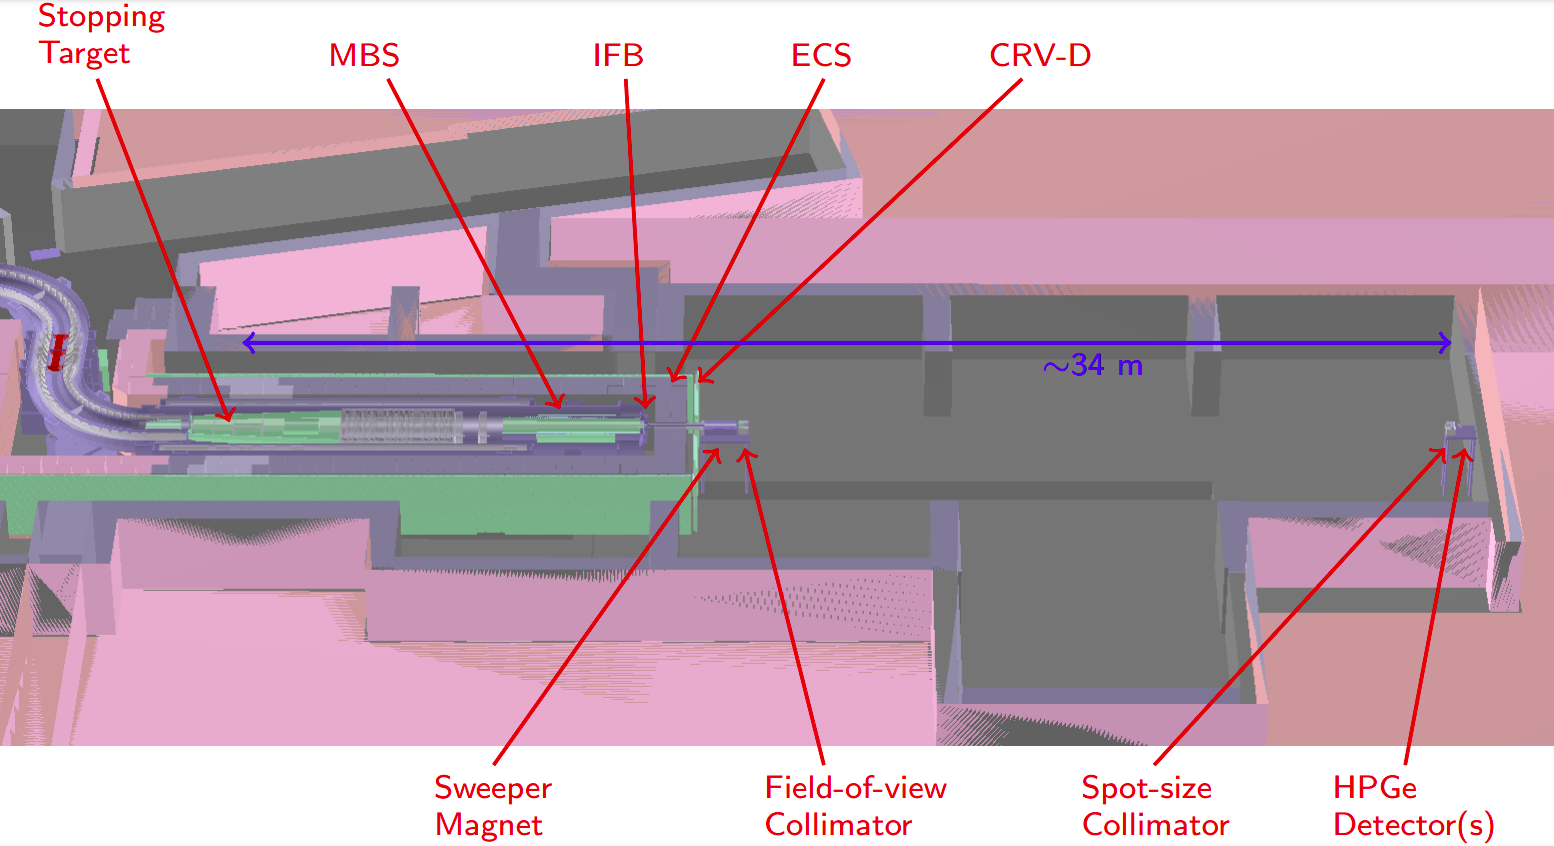
\includegraphics[width =0.7\textwidth]{figures/png/Screenshot_20240306_180910.png}
    \caption[The Stopping Target Monitor geometry.]{The STM geometry showing the DS region (left), 
    the End Cap Shielding, sweeper magnet and STM field-of-view collimator. 
    At the far end of the hall (right) is the final $spot-size$ collimator and the STM detector.}
    \label{fig:stm}
    \end{figure}
    The STM measurement technique exploits the 347 keV X-ray line produced in the 2p$\rightarrow$1s 
    radiative transition of the muon moving to the ground state in the muonic atom (Figure \ref{fig:stmprocess}), 
    which is present for 80\% of the stopped muons. Although the 2p$\rightarrow$1s transition has the 
    largest yield, there are also additional X-ray transitions with substantial yields, 
    including 3p$\rightarrow$1s and 4p$\rightarrow$1s. In addition, the 3d$\rightarrow$2p 
    transition that populates the 2p state appears in the energy spectrum.

    An alternative option is to measure gamma rays associated 
    to muons interactions in the ST (Figure \ref{fig:stmprocess}).
    These are unambiguous signals that muons stopped in the aluminum target. 
    The main signatures are the following ones: 
    \begin{itemize}
    \item 1809 keV gamma-ray that is emitted in the nuclear capture chain:
    \begin{equation}
        \mu^- \ + \ ^{27}\text{Al} \ \rightarrow \ ^{26}\text{Mg}^* \ + \ \nu_\mu \quad \quad ^{26}\text{Mg}^* \ \rightarrow ^{26}\text{Mg} \ + \ \gamma(1809 \ \text{keV})
     \end{equation}
     The $^{26}\text{Mg}^*$ mean de-excitation time is negligible (476 fs) with 
     respect to the muonic atom lifetime (864 ns). 
     This process occurs for 51\% of the nuclear captures.
     \item  A 844 KeV gamma-ray coming from the decay of 
       long-lived ($\tau \sim$9.5 min) isotopes produced in muon nuclear captures:       
     \begin{equation}
        ^{27}\text{Mg} \ \rightarrow \ ^{27}\text{Al} \ + \ \gamma(844 \ \text{keV}) \ + \ e^- \ + \ \bar{\nu}_e
     \end{equation}
     This process occurs for the 9.2\% of nuclear captures.
\end{itemize}

\begin{figure}[!h]
    \centering
    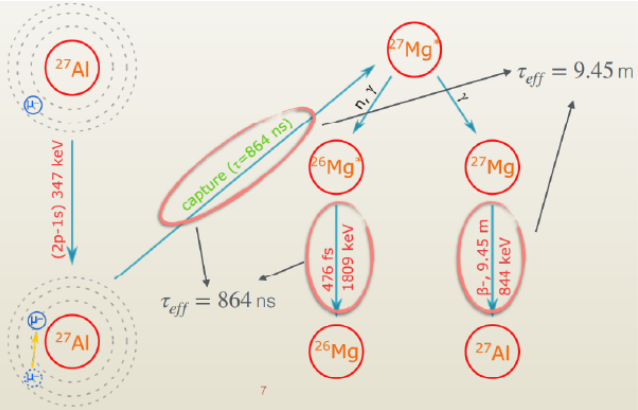
\includegraphics[width =0.6\textwidth]{figures/png/Screenshot_20240706_094517.png}
    \caption[The muon stops 
    and nuclear captures detection in Al ST.]{Reactions that can be exploited to detect the muon stops 
    and nuclear captures in the Aluminum ST.}
    \label{fig:stmprocess}
    \end{figure}

    The Mu2e STM has been designed to determine the number of 
    muons in the ST within 10\% precision over the course of the experiment.  
    It is made of two solid state High Purity Germanium (HPGe) crystal detectors and one 
    scintillating lanthanum bromide (LaBr$_3$) detectors. The HPGe detectors have the 
    energy resolution (FWHM) of 2.5 keV in the energy range of 300-2000 keV and are used 
    to measure photons produced by the secondary muonic aluminium orbital transitions 
    (347 keV) and nuclear captures (884 keV). The LaBr$_3$ detector has an order of 
    magnitude worse energy resolution than the HPGe detector, but it provides a much 
    higher rate capability. It is used to detect prompt photons produced
    in the nuclear captures (1809 keV).  
    \begin{figure}[!h]
        \centering
        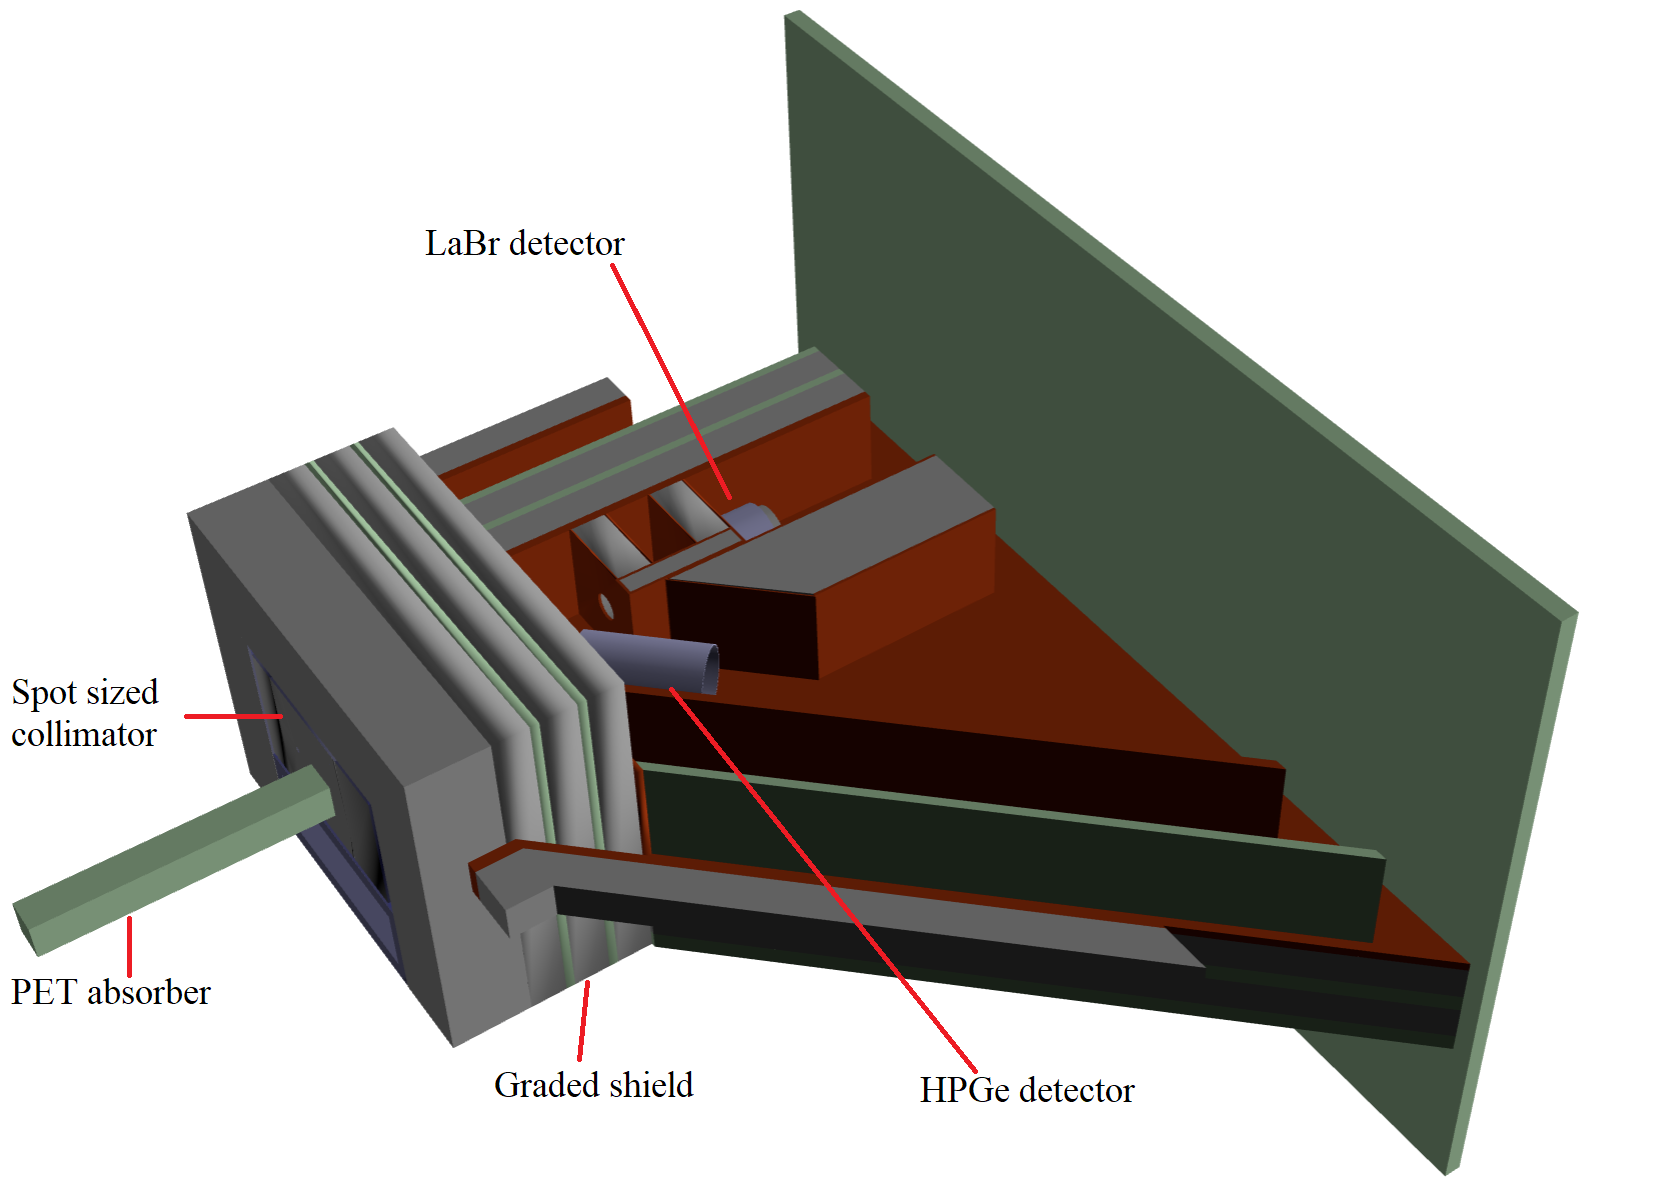
\includegraphics[width =0.4\textwidth]{figures/png/Setup.png}
        \caption[The Stopping Target Monitor geometry.]{The STM geometry.}
        \label{fig:stmfigure}
        \end{figure}
The STM geometry is shown in Figure \ref{fig:stmfigure}.




